\documentclass[french,a4paper,12pt]{report}
\usepackage[utf8]{inputenc}
\usepackage[T1]{fontenc}
%\Package paramétrage: marge horizontale à 2,5 cm, et la marge verticale à 1,5 cm.
\usepackage{geometry}
\geometry{hmargin=2cm,vmargin=3cm}
\usepackage{eso-pic}
\usepackage{graphicx}
\usepackage{float}
\usepackage{listings}
\usepackage{color}
\definecolor{dkgreen}{rgb}{0,0.6,0}
\definecolor{gray}{rgb}{0.5,0.5,0.5}
\definecolor{mauve}{rgb}{0.58,0,0.82}
\usepackage{pdfpages}

\lstset{frame=tb,
  language=Java,
  aboveskip=3mm,
  belowskip=3mm,
  showstringspaces=false,
  columns=flexible,
  basicstyle={\small\ttfamily},
  numbers=none,
  numberstyle=\tiny\color{gray},
  keywordstyle=\color{blue},
  commentstyle=\color{dkgreen},
  stringstyle=\color{mauve},
  breaklines=true,
  breakatwhitespace=true,
  tabsize=3
}

%\hfill\hbox to 0pt{\hss
\includegraphics[width=7cm]{UTBM_LOGO.png}\hss}\hfill\null\newline

\begin{document}

\title{	Université de Technologie de Belfort-Montbéliard \\
		{\large \textsc{Génie logiciel, spécialisé dans les systèmes embarqués }} \\
		\vspace{1cm}
		Laboratoire de Physique Nucléaire et des Hautes Énergies \\
		{\large \textsc{Contrôle Haptique et Asservissement de la Mécanique des Pianos de concert }}		
	  }
	  
\date{5 Février 2018 -- 13 Juillet 2018 }
	  
\author{Professeur suiveur : GECHTER Franck  \\
		Tuteur de stage		: LEBBOLO Hervé  \\
		Elève				: ROMET Pierre
		}

\makeatletter
  \begin{titlepage}
  \centering
  \
      {\large \textsc{ }}\\
      \textsc{}\\
      
      \vfill
       {\LARGE \textbf{\@title}} \\
    	\vspace{2em}     
      
    \vspace{1cm}
      {\large{	\@date\\
    \vspace{1cm}
       Stage ST50}}\\
    \vspace{1cm}
        {\large \@author} \\
    \vfill
        
\includegraphics[height=0.13\textheight]{UTBM_LOGO.png}
        \hfill
        
\includegraphics[height=0.09\textheight]{LPNHE_LOGO.png}
  \end{titlepage}
\makeatother

\tableofcontents
\parskip=5pt %to redefine line space of text only, and not for "tableofcontents"


%--------------------------------------------------------------------------------------
%
%	Avant Propos
%
%--------------------------------------------------------------------------------------
\part{Préambule}

  \chapter{Remerciement}
  Tout d'abord je tiens à remercier l'ensemble de mes collègues pour l'accueille des plus chaleureux, au sein du laboratoire de physique nucléaire et des hautes énergies, ainsi que pour leur présence tout au long de mon stage, en m'aidant et me conseillant.
  
  Je voudrais remercier Monsieur Olivier LEDORTZ pour son aide concernant le langage VHDL.
  
  Je tiens à remercier mon maitre de stage Monsieur Hervé LEBBOLO, pour son implication dans l'encadrement de mon stage, son soutien, ainsi que pour l'ensemble des connaissances transmises dans le domaine de l'électronique analogique.
  
  Enfin, je tiens également à remercier mon enseignant suiveur, Monsieur Franck GECHTER, grâce à qui j'ai pu réaliser un stage de fin d'étude me permettant d'allier mon corps de métier, à une passion, la musique.
  
 \chapter{Introduction}

Dans le cadre des mes études d'ingénieurs au sein de l'Université de Technologie de Belfort-Montbéliard, j'ai effectué un stage de fin d'étude en laboratoire d'une durée de 24 semaines au sein du Laboratoire de Physique Nucléaire et des Hautes Énergies à Paris.

Le laboratoire de Physique Nucléaire et des Hautes Énergies est une unité de recherche de l'institut national de  physique nucléaire et de physique des particules, institut du CNRS et des universités Sorbonne Université et Paris Diderot.

Mon stage s'est déroulé au sein du service électronique, sous la tutelle de Monsieur Hervé LEBBOLO.

Lors de ce stage, je fut recruté pour participer au projet "CHAMP"; projet interdisciplinaire, initié par Antoine LETESSIER SELVON, Hervé LEBBOLO, Philippe REPAIN, Laurent BESSIER, Thomas Hélie.

Ce projet interdisciplinaire associe de nombreuses compétences, en lutherie artisanal, en technique de préparation de piano, en physique, en électronique rapide et en mécanique de précision.

L'objectif est la réalisation d'un système de motorisation asservie de la mécanique d'un piano à queue afin d'offir de nouvelles couleurs aux préparateurs de pianos, ainsi que de nouvelles voies d'expression musicales aux interprètes tout en gardant intact le toucher traditionnel des mécaniques à répétition.

Le laboratoire étant spécialisé dans le domaine de l'électronique de précision et de l'éléctronique numérique, travaillant sur des projets tel que LSST (Large Synoptic Survey Telescope - Grand téléscope d'étude synoptique), ce stage fut pour moi l'occasion d'évoluer dans un domaine des systèmes embarqués que je ne maitrisais peu, (de part ma formation) l'électronique analogique et numérique, ce qui m'as permis de découvrir et d'acquérir de nouvelles compétences ainsi que les méthodes de développement qui y sont lié.

Suite à cette introduction, nous allons poursuivre avec la présentation du laboratoire (LPNHE), puis nous conclurons cette premières partie par la présentation du projet "CHAMP".


  
	\chapter{Présentation du laboratoire}
  Le LPNHE a été fondé par un groupe de chercheurs et enseignants-chercheurs issus de la division « hautes énergies » de l’institut de Physique Nucléaire (IPN) d’Orsay. En 1970, ces spécialistes des chambres à bulles rejoignent l’université Paris VI, puis l’ensemble devient un laboratoire associé au CNRS. A cette époque, la recherche s’y organise principalement autour d’expériences de chambres à bulles au CERN. Le LPNHE a donc derrière lui une longue histoire de collaboration avec le CERN.e
  
  Aujourd’hui encore, même si les expériences et projets dans lesquels est engagé le laboratoire se trouvent maintenant sur les cinq continents, le CERN reste l’endroit privilégié où les chercheurs de physique des particules du laboratoire effectuent leur recherche.
  
  Le Laboratoire de Physique Nucléaire et des Hautes Énergies est une unité de recherche de l'institut National de Physique Nucléaire et de Physique des particules, institut du CRNS et des universités Sorbonne Université et Paris Diderot. Il est constitué de 12 groupes de recherche, dont un à l’interface physique/biologie, de 3 services techniques (informatique, électronique, mécanique), et de deux services support étant l'administration et la logistique.
  
  Ces programmes couvrent les enjeux actuels de la physique des particules, des astroparticules, et de la cosmologie.
  On retrouve un groupe constitué de:
  \begin{itemize}
  \item  24 enseignant chercheurs
  \item  27 chercheurs
  \item  44 personnels d'appuis à la recherche
  \item  20 Doctorants
  \end{itemize}
  \newpage
  
  \section{Présentation des activités}
  Le Laboratoire de physique nucléaire et des hautes énergies (LPNHE) est engagé dans plusieurs grands programmes expérimentaux, poursuivis dans le cadre de collaborations internationales auprès de très grandes infrastructures de recherche du monde entier, tel que des centres d’accélérateurs de particules, ainsi que des observatoires. Ces programmes couvrent les enjeux actuels de la physique des particules, des astroparticules, et de la cosmologie :
  
  On retrouve ainsi des travaux portant sûr:  
  \begin{itemize}
  \item L'origine des masses et des familles de particules, recherche du boson de Higgs, unification des interactions fondamentales, recherche de la supersymétrie, dimensions supplémentaires de l’espace-temps : thèmes abordés par les expériences CDF et D0 auprès du Tevatron à Fermilab, et par des expériences auprès du Large Hadron Collider au CERN (ATLAS au LPNHE), et enjeux d’un futur collisionneur e+e- pour lequel le LPNHE est engagé dans le développement de détecteurs en silicium.
  
  \item L’asymétrie matière-antimatière et la physique des saveurs lourdes : ce sont les sujets principaux des expériences BaBar au « SLAC National Laboratory », LHCb au CERN et la future SuperB factory en Italie.
  
  \item Les propriétés des neutrinos : participation à l’expérience Tokaï To Kamiokande (T2K) au Japon.
  
  \item Le contenu énergétique de l’univers, matière noire et énergie noire : le groupe Cosmologie du LPNHE joue un rôle déterminant dans Supernovae Legacy Survey (SNLS) auprès du Canadian French Hawaï Telescope dans Supernovae Factory (SNF) et est engagé dans la préparation des projets futurs Large Synoptic Survey Telescope (LSST) et EUCLID.
  
  \item L'origine des rayons cosmiques de très haute énergie : rayons gamma au TeV pour l’observatoire HESS en Namibie, et rayons cosmiques d’ultra haute énergie (10**18 eV) pour l’observatoire AUGER en Argentine.
  \end{itemize}
  
  Depuis la conception des expériences, en passant par l’étude et la réalisation des instruments de détection, la mise au point des systèmes de détection, d’acquisition et de réduction des données, la calibration et le monitorage des détecteurs pendant les longues périodes de prise de données, l’analyse et l’interprétation physique des mesures, pour enfin aboutir aux publications.
  Ce travail s'étale sur plusieurs années, parfois plus de dix ans, réunissant des équipes et développent des compétences extrêmement diversifiées en physique, électronique, informatique ou mécanique. 
  Les théoriciens du LPNHE représentent une petite composante qui enrichit la vie scientifique du laboratoire, ainsi que de la Fédération de Recherche sur les Interactions Fondamentales (FRIF), dont le laboratoire est membre, ce qui favorise un rapprochement plus fort théoriciens-expérimentateurs.
  
  \newpage
  
  \section{Projet et thématique}
  Voici quelques exemples de projets sur lesquels les équipes du laboratoire sont engagés:
  \begin{itemize}
  \item Physique des particules: Frontière en énergie
  
  	- L'expérience Atlas, au LHC (Cern), est l'un des deux détecteurs polyvalents du grand collisionneur de hadrons (LHC). Il étudie des domaines de de physique très variés, de la recherche du boson de higgs, aux dimensions supplémentaires de l'espace-temps, en passant par les particules qui pourraient former la matière noire.
  	
  \begin{figure}[!ht]
    \center
    %\hfill\hbox to 0pt{\hss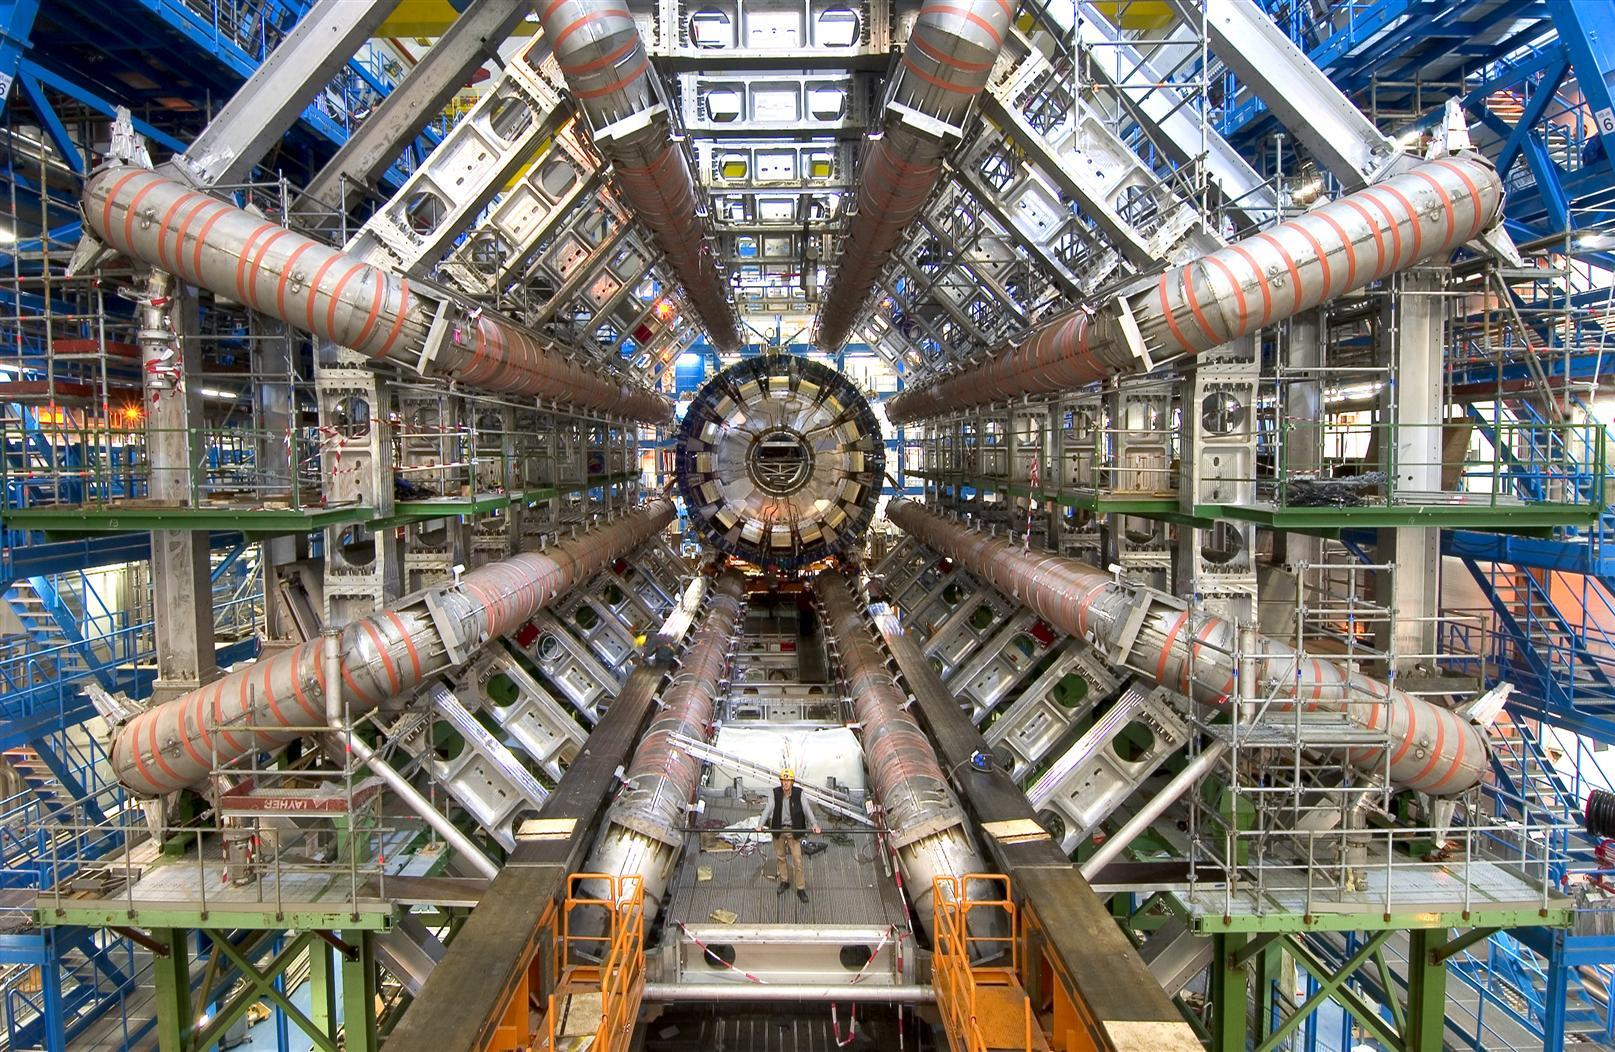
\includegraphics[width=10cm]{ATLASLHC.jpg}\hss}\hfill\null\newline
    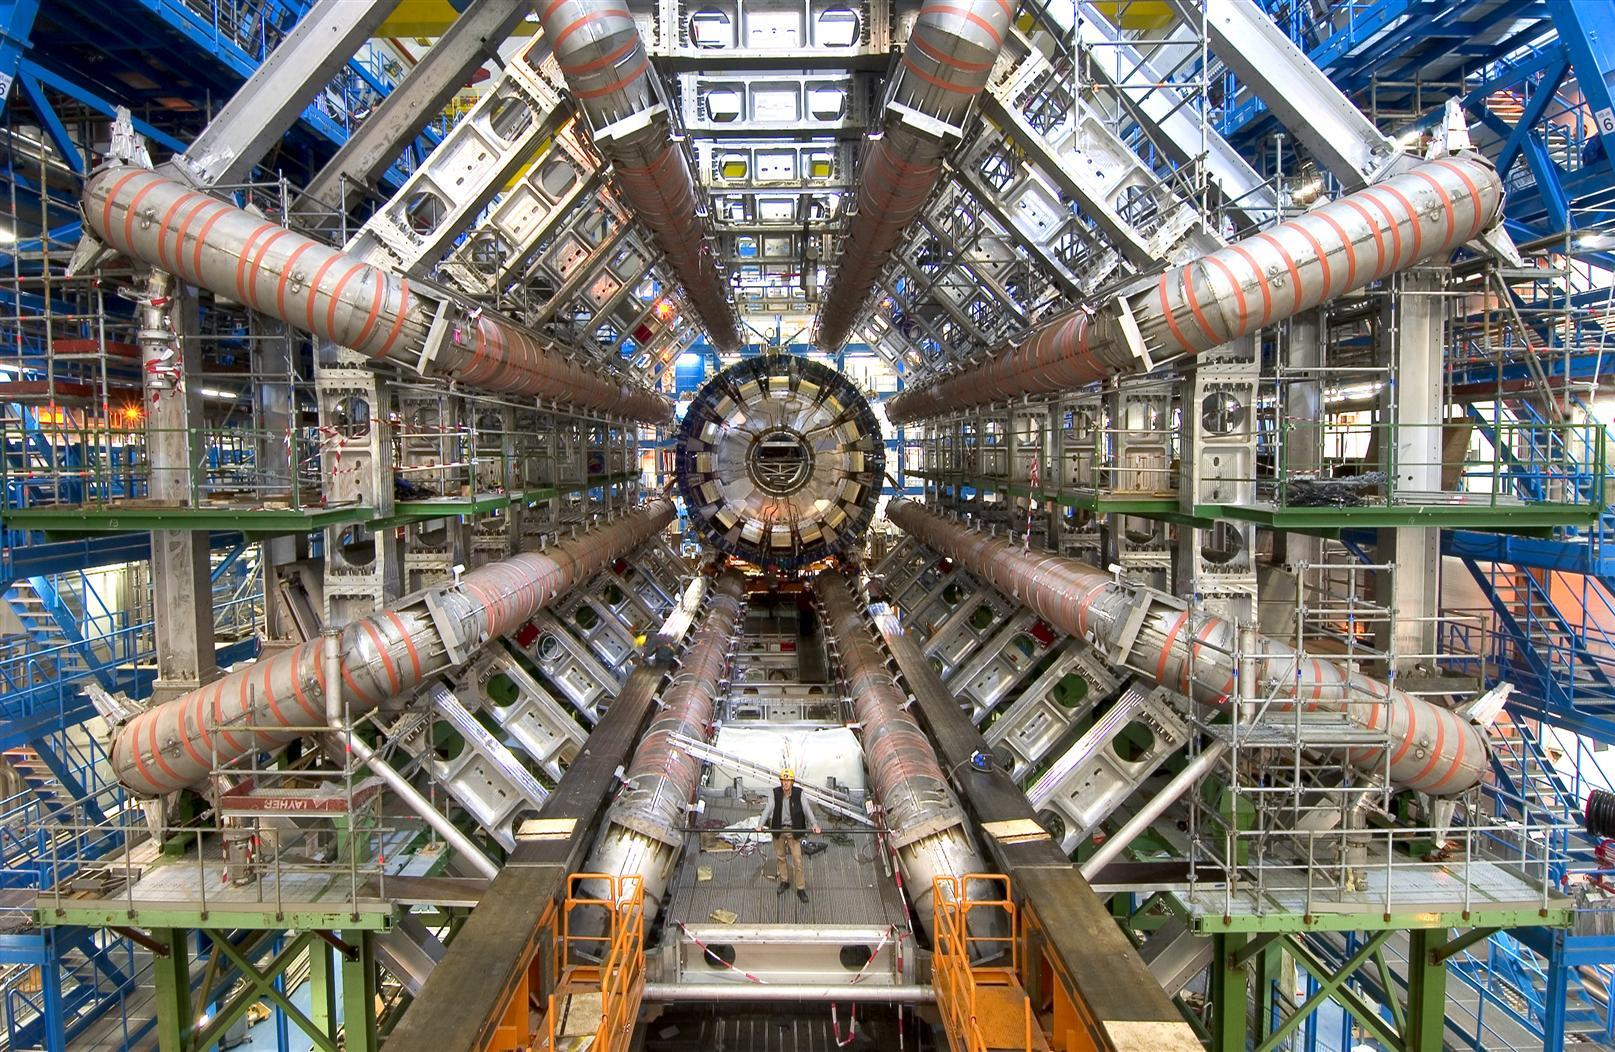
\includegraphics[width=9cm]{ATLASLHC.jpg}
    \caption{Expérience Atlas}
	\end{figure}
  	
 	
 	- L'expérience CDF pour "Collider Detector at Fermilab" met en jeux un accélérateur de particule, nommé le "Tevatron", faisant accélérer et se collisioner, des prontons ainsi que des antiprotons. 	Il à pour but d'observer et de découvrir l'identité ainsi que les propriétés des particules qui compose l'univers, et de comprendre les interactions entre ces dernières.
 	CDF est en particulier connue pour la d"couverte du "Quark Top" en 1994, confirmé par l'expérience "D0" l'année suivante.
 	
	\begin{figure}[!ht]
    \center
    %\hfill\hbox to 0pt{\hss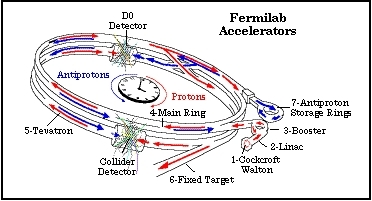
\includegraphics[width=11cm]{D0.jpg}\hss}\hfill\null\newline%
    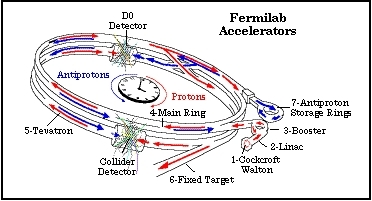
\includegraphics[width=11cm]{D0.jpg}
    \caption{Expérience CDF (Collider Detector at Fermilab)}
	\end{figure} 
 	
  \item Physique des saveurs:
 
	- "T2K" pour Tokai to Kamioka est une expérience de physique des particules situé au japon, dans laquelle collabore de nombreux pays. Il s'agit d'une expérience d'oscillation de neutrinos, mesurant un faisceau de neutrinos muoniques à courte (280 m) et longue distance (295 km). 
	Le but principale de T2K est de mesurer l'oscillation des neutrinos muoniques en neutrinos électroniques afin de mesurer le derniers paramètre de la matrice "Pontecorvo-Maki-Nakagawa-Sakata" permettant d'expliquer l'oscillation deneutrinos prédite par Bruno Pontecorvo en 1957.	
	
  	-"SLAC" ou "BABAR", est une expérience de physique des particules réalisé au Stanford Linear Accelerator Center. Elle est dédiée à létudes de la physique des mésons B et de la violation de la symétrie CP dans leur désintégration faibles.
  	
  	\textsc{\begin{figure}[h]
     \begin{minipage}[c]{.46\linewidth}
         \centering
         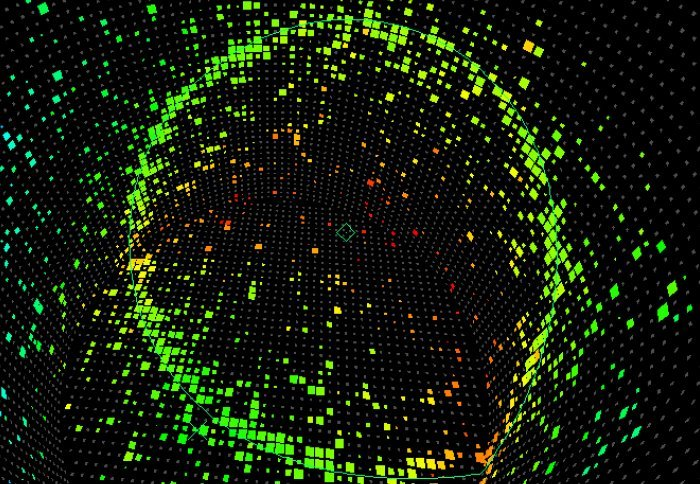
\includegraphics[width=4cm]{T2K.jpg}
         \caption{Expérience T2K (Tokai to Kamioka)}
     \end{minipage}
     \hfill%
     \begin{minipage}[c]{.46\linewidth}
         \centering
         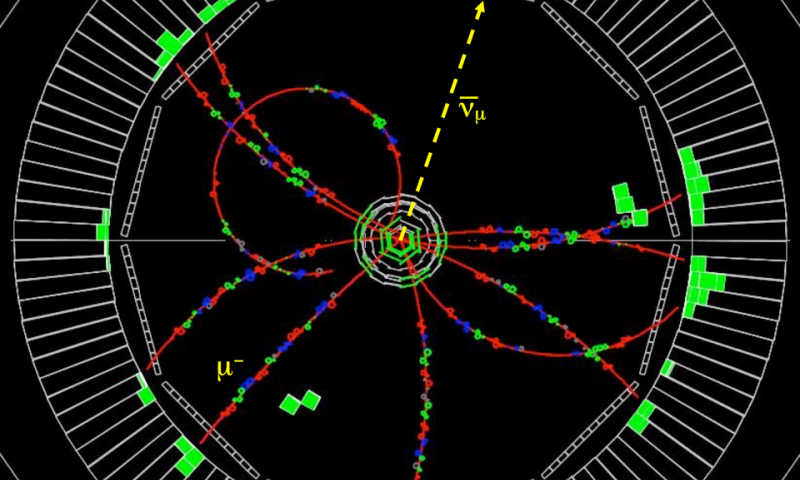
\includegraphics[width=5cm]{SLACBABAR.png}
         \caption{Expérience SLAC (ou BABAR)}
     \end{minipage}
 	\end{figure}} 	
  
  \item Cosmologie:
  
  Le compréhension de la nature, de le matière et de l'énergie noires nécessite de mesurer les paramètres cosmologiques avec une précision de l'ordre du pourcent. Les mpyens à mettre en oeuvre pour atteindre cet objectif passent par l'échantillonnage de très grandes portions de l'univers visible. A cette fin, il faut non seulement pouvoir observer à grande distance, mais avec un dispositif à très grand champ.
  
  Pour cela, le projet au sol "LSST", vise à l'observation répétée de l'ensemble du ciel visible, en s'affranchissant d'une partie des effets instrumentaux et atmosphérique. Il est basé sur un télescope au sol de 8.4 mètres de diamètre équipé d'une caméra de 3.2 milliard de pixels. L'ensemble, implanté au Chili, couvrira un champ de 9.6 degrés-carrés sur le ciel balayé à la cadence d'un champ toutes les 40 secondes. Chaque champ sera ainsi visité 1000 fois durant les 10 ans de prise de données du programme.\newline
    	
	\begin{figure}[!ht]
    \center
    %\hfill\hbox to 0pt{\hss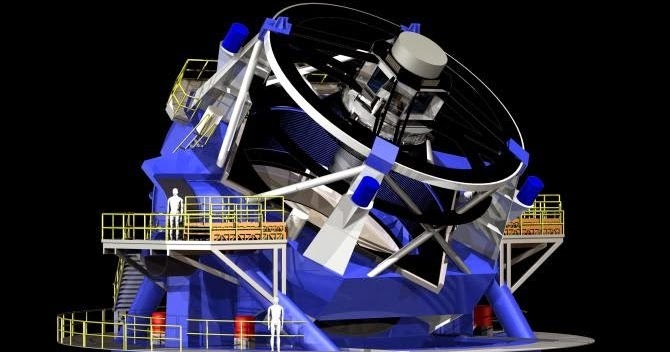
\includegraphics[width=8cm]{lsst.jpg}\hss}\hfill\null
    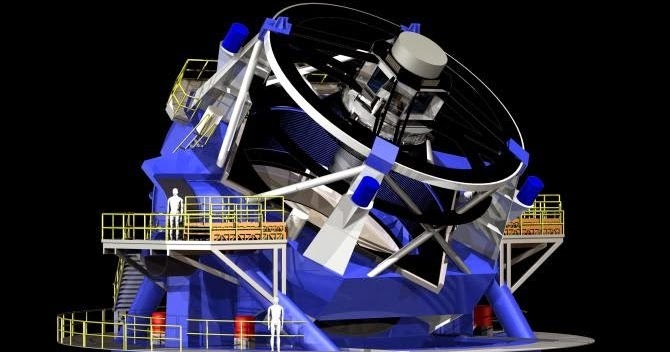
\includegraphics[width=5cm]{lsst.jpg}
    \caption{Projet LSST (Large Synoptic Survey Telescope)}
	\end{figure} 
		  	
  \end{itemize}
  
    
%--------------------------------------------------------------------------------------
%
%	Présentation du projet "CHAMP"
%
%--------------------------------------------------------------------------------------
\part{Qu'est ce que le projet "CHAMP" ?}
  \chapter{Présentation}
  
  Ce projet est né de la rencontre de Laurent BESSIÈRES, préparateur de piano intervenant pour les concerts et récitals de la Philarmonoe de Paris, et de Antoine LETESSIER SELVON, physicien des hautes énergies, directeur de recherche au CNRS et pianiste amateur. 
  
  De leur discution est né un projet au travers du quel ils cherche à élargir les possibilités de l'instrument en modifiant de mainère original sa mécanique. C'est en s'appuyant sur des techniques modernes qu'il souhaite proposer de nouveaux moyen d'expression aux artistes, tout en respectant le lien étroit qu'ils entretiennent avec leur instrument nottament au travers du toucher.
  
  \section{État de l'art}
  
  C’est en 1700 que Bartolomeo Cristofori invente la mécanique à échappement et construit le premier instrument à cordes frappées : le piano-forte. Ce sont les balbutiements de l’histoire du piano à queue. Le piano-forte révolutionne la technique pianistique car il permet à l’interprète de passer par le jeu des doigts, d’une nuance piano à une nuance forte, ouvrant de nouvelles voies à l’expression musicale et à la créativité des compositeurs. Cent vingt-trois ans plus tard, en 1821, Sébastien Érard ajouta un système de répétition à la mécanique de Cristofori et invente la mécanique moderne dite (improprement) à double échappement.

A la même époque, deux progrès techniques et industriels vont donner naissance au piano moderne. D’une part l’utilisation d’acier fondu pour les cordes et d’autre part l’introduction de cadres métalliques en fonte. Par ailleurs, de nombreux brevets seront déposés concernant la table d’harmonie, le croisement des cordes, le chevalet, l’assemblage de la mécanique, etc. 

De telle sorte, que peu avant 1890, l’essentiel de ce qui fait un piano moderne est accompli. A partir de cette date et à la suite d’une concentration industrielle de plus en plus forte, la nécessité de produire le plus d’instruments possible au moindre coût pour garantir plus de parts de marchés, les innovations vont essentiellement cesser et conduire en moins d’un siècle à la disparition de presque tous les facteurs artisanaux et à l’uniformisation quasi totale des instruments avec pour référence le piano de concert Steinway dont le modèle produit en 1877 réunissait déjà les inventions les plus importantes du XIXe siècle.

\newpage
On peut légitimement se demander quelles sont les lacunes du Steinway d’aujourd’hui, joué par 95\% des pianistes de la planète, qui justifieraient de bouleverser l’état actuel.
De fait, nous ne souhaitons pas nous appuyer sur d’éventuelles lacunes du Steinway ou d’ailleurs de tout autre piano, nous voulons avant tout ouvrir de nouvelles pistes. 
 Ceci en introduisant une source extérieure d’énergie, totalement et délicatement pilotée par l’instrumentiste, nous allons libérer des contraintes auquelles les pianos modernes, les Steinway en particulier, ont répondu de manière optimale, mais qu’ils ont malgré tout intégré.
 
 \section{Motivations}
 
 La mécanique à répétition de Sébastien Érard, brevetée à Londres par son neveu Pierre en 1921, est toujours utilisée aujourd’hui. Pourtant, la demande contemporaine de piano de concerts d’une puissance toujours plus grande (sans perte de sensibilité) n’a jamais été aussi forte. Par ailleurs, au cours des 30 dernières années, des facteurs indépendants ont introduit des innovations (nouveaux alliages pour les cordes, nouvelle structure pour le cadre et la table d’harmonie, etc) et repensé certains des choix techniques de la fin du XIXe siècle (croisement des cordes, barrage,...). Ainsi en France, Stephen Paulello, le dernier facteur français de pianos de concert en activité, vient de produire le premier exemplaire de sa dernière création : l’Opus 102. Ce piano de concert fait 3m de long et possède une tessiture de 102 notes (contre environ 2m80 et 88 notes pour les pianos de concert standard). Il comporte de nombreuses innovations et a été accueilli par la critique comme la “Bugatti Royale” des pianos.

La mécanique, de son coté, a peu évolué. L’utilisation de matériaux composites ou la modification de certaines pièces a parfois permis d’explorer quelques pistes (légèreté, coût, endurance, reproductivité) mais de manière limitée car le compromis actuel semble optimal compte tenu des contraintes imposées par la morphologie de l’instrument et de l’énergie qu’un artiste peut raisonnablement fournir pour l’actionner. Compte tenu de ces contraintes, l’ouverture vers de nouvelles expressions sonores par le biais de la mécanique ne semble pas
avoir été explorée. Certains développements ont consisté à introduire des éléments passifs, aimants, ressorts, élastiques, à l’intérieur de la mécanique ou sous les touches, mais aucun n’a semblé apporter suffisamment pour emporter l’adhésion des techniciens et surtout des artistes.\newline

	\begin{figure}[!ht]
    \center
    %\hfill\hbox to 0pt{\hss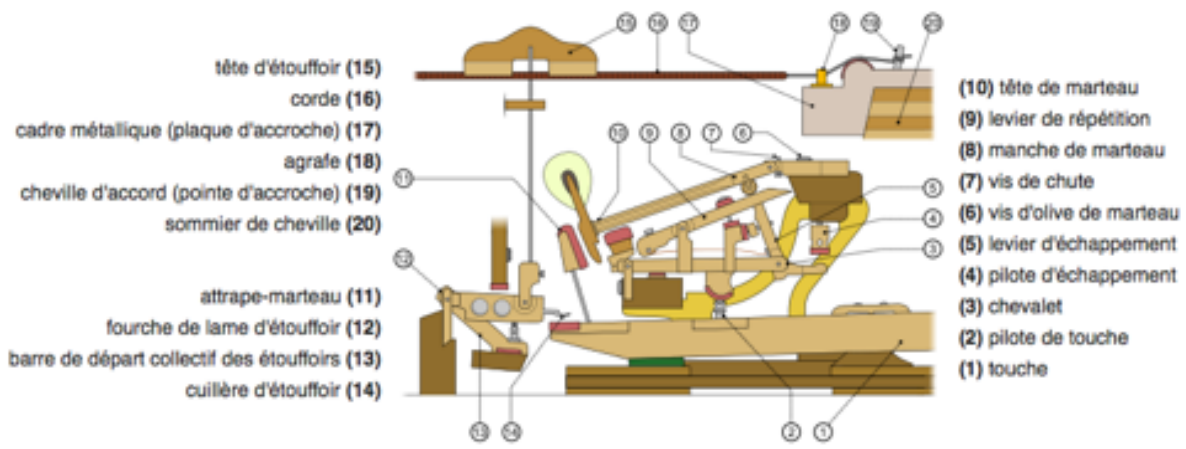
\includegraphics[width=15cm]{MECA_PIANO.png}\hss}\hfill\null
    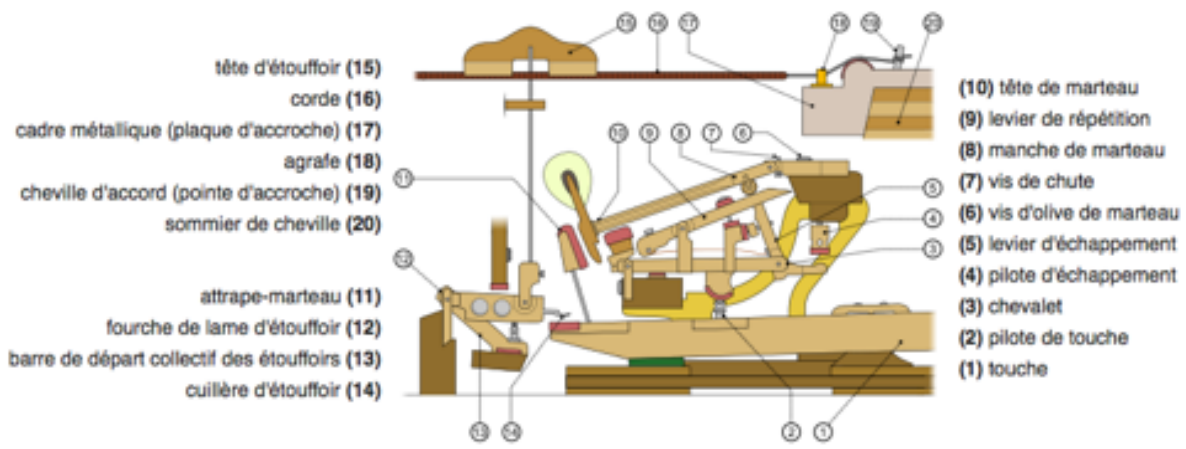
\includegraphics[width=15cm]{MECA_PIANO.png}
    \caption{Schéma de mécanique de Piano}
	\end{figure} 

Côté éléments actifs, l’essentiel des innovations concerne la reproduction autonome par l’instrument d’une musique jouée précédemment (sur lui même ou sur un instrument similaire), c’est la cas par exemple de la technologie "DisklavierTM" mise au point par Yamaha. Il n’y a pas d’interaction directe entre l’artiste et la mécanique augmentée. La mécanique de ces pianos enregistre le jeu de l’artiste puis le restitue sans son aide, avec une
perte de sensibilité notable. Il n’y a donc pas d’exploration de nouvelles capacités sonores ou d’augmentation de la palette de couleur de l’instrument, bien au contraire. Notons cependant les explorations de certains chercheurs comme par exemple Andrew McPherson6 et son “Magnetic Resonator Piano” où des électroaimants placés au dessus des cordes les maintiennent en résonance sous le contrôle de l’interprète offrant ici très clairement de nouvelles options d’expression.

D’un autre côté, les salles de concerts sont de plus en plus grandes et demandent, malgré une acoustique souvent exceptionnelle, des instruments de plus en plus puissants. Notons également que les orchestres sont aussi plus larges et que les instruments eux-mêmes, des cordes aux cuivres, ont également gagné en puissance. Ainsi on trouve aujourd’hui des pianos de plus de 3m (Fazioli 3,08m) permettant en principe d’obtenir une puissance extrême mais
c’est toujours la mécanique de Sébastien Érard qui est employée pour produire le son, une mécanique à la puissance limitée par celle que l’artiste peut lui fournir.

La puissance n’est cependant que l’un des paramètres sur lequel l’addition d’une source extérieure d’énergie permet d’intervenir. À puissance fixe, on peut explorer une répartition différente de l’énergie cinétique entre la masse du marteau et sa vitesse. Cette exploration est très limitée dans le cas d’une mécanique traditionnelle car l’inertie de l’ensemble doit être contenue afin que l’effort d’enfoncement des touches reste tolérable pour l’artiste, surtout à haute vélocité. Il en ressort que les masses des marteaux et le point de frappe, deux éléments qui ont une importance considérable dans la couleur du son, indépendamment de la dynamique, sont aujourd’hui fixés à des valeurs de référence choisies et considérées comme optimales par le fabricant dominant le marché actuel et pour l’essentiel copiées par tous les autres. Insistons néanmoins sur le fait que compte tenu des contraintes décrites ci-dessus
(inertie, poids, morphologie), les variations sur ces paramètres sont très limitées, et c’est pourquoi nous nous proposons de lever une partie au moins de ces contraintes.

Ce constat est aussi celui que fait Laurent Bessières qui, après avoir exercé son métier d’accordeur préparateur concert pendant plus de 15 ans auprès des plus grands artistes et dans les plus grandes salles de concert de Paris, aimerait pouvoir offrir d’avantage à ceux qui le souhaitent. Les artistes ont en effet des exigences quant au toucher et à la sonorité souvent contradictoires compte tenu de ce qui peut être fait sur une mécanique ordinaire. Une plus grande latitude dans le mode de transfert d’énergie de la touche au marteau et du marteau à la corde permettrait une exploration d’une palette de couleurs beaucoup plus large et également une meilleure exploitation des nouvelles technologies de cadres et de cordes.

\section{Concepts} 

La mécanique des pianos à queue (figure 1) est constituée de trois pièces principales : la touche, le chevalet et le marteau. Lorsque la touche est enfoncée, elle transmet l’énergie du doigt qui l’enfonce au chevalet qui démultiplie la vitesse d’enfoncement afin de propulser à grande vitesse (jusqu’à plusieurs m/s) le marteau sur les cordes. Les réglages de la mécanique permettent de modifier la sensation de toucher et la production sonore. Ainsi, on peut obtenir un clavier plus léger ou plus lourd et un son plus puissant, plus doux, plus clair ou plus feutré.

Le transfert d’énergie des marteaux aux cordes passe par une impulsion mécanique dont l’amplitude dépend de l’énergie cinétique du marteau (l’énergie cinétique est proportionnelle au produit de la masse du marteau par le carré de sa vitesse) et dont la durée (à vitesse de marteau fixée) dépend de la dureté des feutres, du point de frappe et de l’élasticité des cordes. Les mécaniques standards imposant la masse des marteaux et le point de frappe, le préparateur ne peut jouer pour l’harmonisation que sur les feutres tandis que l’énergie maximale transmise est, toutes choses égales par ailleurs, fixée par la masse du marteau lui même.

De nombreux articles, rédigés par des spécialistes, concluent (sur la base de leurs expériences) que le poids des marteaux est un élément essentiel de l‘harmonie du piano :

\begin{itemize}
	\item  “Le poids du marteau n'a pas seulement une grande incidence sur le toucher, il en a aussi une sur le son. En ce sens, nous devons bien inclure l'effet sonore du poids du marteau dans toute discussion au sujet du réglage du toucher”; c.f. Boddin Piano Service.

	\item  “[...] appréciation critique d'un piano à queue steinway modèle S: les marteaux étaient légers, le son semblait irréprochable. Franz accrocha des poids de quelques grammes sur quelques manches de marteau et déplaça ainsi le dit poids dans la "high zone” [région désignant les pianos dits lourds, NDLR]. A I'écoute du son ainsi modifié, leur surprise fut
très grande: ça n'était plus seulement du son, on pouvait carrément sentir le son occuper l'espace. La différence fut si importante que Wim s'exclama : " Mais alors, c'est quoi l'intonation !?" Ses mots nous interpellèrent tous. Voilà qui prouve que nous avons bien à réexaminer en profondeur l'idée et la pratique de l'intonation en y intégrant le rôle que
joue le poids du marteau, [...]”.

	\item  “D'une façon générale, la majorité des améliorations successives ont toutes cherché à obtenir un son à la fois fort et tenu. La sonorité des pianos actuels donne l'illusion d'une continuité sonore que les facteurs ont toujours cherché à obtenir. A l'inverse, un système élaboré d'étouffoirs permet d'obtenir des sons extrêmement brefs, ce qui fut longtemps impossible. Pour obtenir cette double qualité, la dimension et le poids des marteaux qui viennent frapper les cordes se révèle décisif. [...] Le rapport de la masse de la corde à la masse du marteau se révèle ici le facteur déterminant.” par René Caussé dans Résonance no 5, septembre 1993 Copyright © IRCAM.

\end{itemize}

Le poids d’enfoncement d’une touche de clavier est compris entre 45g et 60g, celui des marteaux est d’un peu moins de 12g dans les basses à moins de 5g dans les aigus, et ce depuis 200 ans. C’est le confort de jeu des pianistes qui l’impose. Pour maintenir l’inertie des touches à un niveau acceptable, il faut également que l’ensemble du poids mis en mouvement ne soit pas trop élevé et donc que le contre-poids (en plomb) mis dans les touches reste faible. Ces deux principes limitent la masse du marteau qui est le seul élément qui pourrait, si on augmentait sa masse, transmettre toute l’énergie qu’un piano de 3m (et plus!) peut développer.



\chapter{Les premières approches}

  \section{Mécanique et Electronique}
Nos premières réflexions sur la réalisation d’un système d’assistance et d’asservissement d’une mécanique de piano à queue démontrent qu’il faut faire appel à des technologies de pointe. Ce qui explique l’aspect novateur de notre projet. Par exemple, les contraintes mécaniques sur les moteurs susceptibles de seconder les doigts dans leur action sont nombreuses. Pour ne citer que les plus essentielles :\newline

	\begin{figure}[!ht]
    \center
    %\hfill\hbox to 0pt{\hss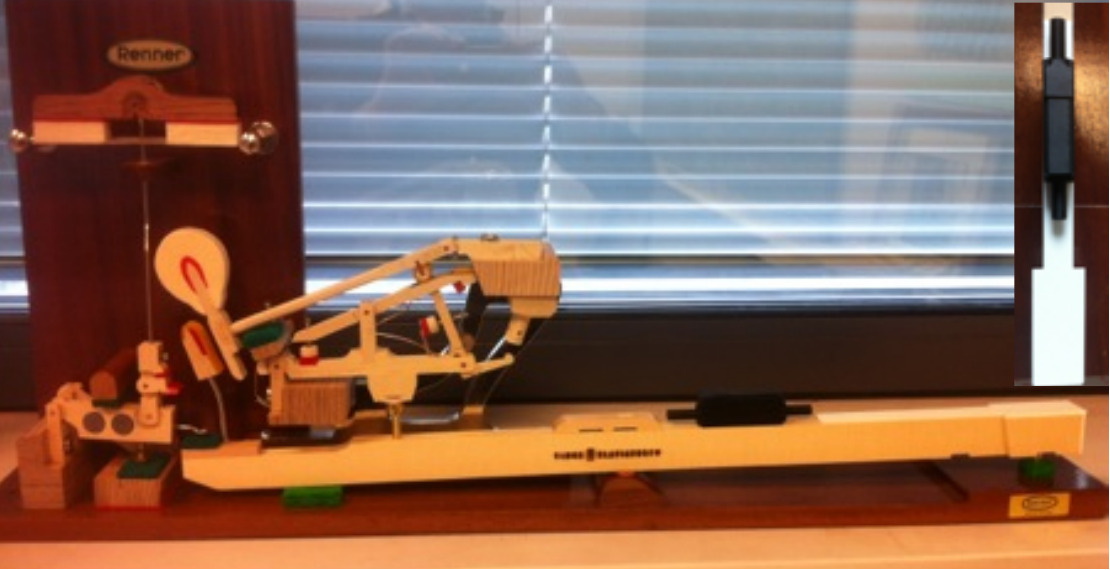
\includegraphics[width=13cm]{MECA_PIANO2.png}\hss}\hfill\null
    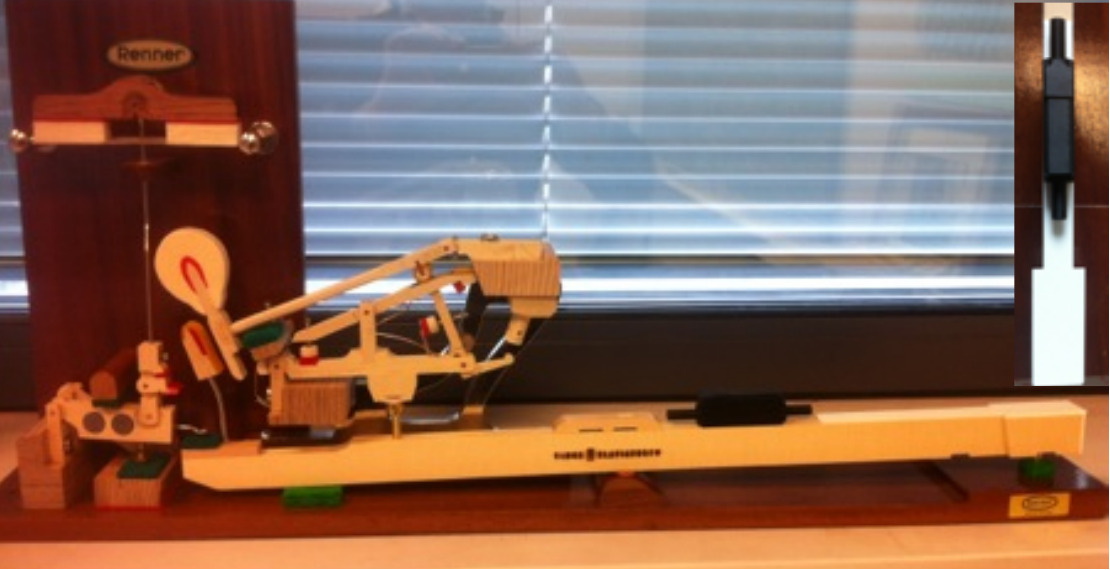
\includegraphics[width=10cm]{MECA_PIANO2.png}
    \caption{Mécanique de Piano}
	\end{figure} 

%Une mécanique de type Renner avec un modèle 3D de l’actuateur linéaire
%envisagé (en noir posé sur la touche) pour donner l’échelle. L’actuateur peut être soit intégré
%dans le sommier en tête de la mécanique sous la cuillère d’étouffoir ou bien positionné à
%l’arrière de celle-ci sur le sommier de cheville. Plusieurs positions seront étudiées. En insert
%une vue de l’actuateur sur la touche qui montre que sa largeur est parfaitement adaptée.

\begin{itemize}
	\item  rapidité : temps de réponse à la milliseconde, vitesse maximum de l’ordre du mètre par
	seconde, accélération de l’ordre de 10 ou 20 g (100 à 200 m/s2 ).

	\item Puissance : force en impulsion de l'ordre de 1kg ou 10N.

	\item encombrement faible: dimension de l'ordre de 1 cm(l) x 1 cm(p) x 5 cm(h).

	\item bruit, inexistant ou négligeable : 10-15 dB à moins de 1m.

	\item précision : positionnement du manche de marteau au dixième (0.1 mm).

	\item fiabilité : durée de vie de milliers d'heures et plus de 10 millions de mouvements.
\end{itemize}

Des moteurs avec ces caractéristiques sont disponibles aujourd’hui et font appel (entre autres) à de puissants aimants miniatures pour les mouvements et à des sondes à effet Hall intégrées pour le positionnement. La figure 5.2 montre un profil de mécanique (c’est a dire la mécanique complète d’une touche individuelle) de la marque Renner, d’autres modèles existent, notamment sur les Steinway, mais leurs caractéristiques essentielles sont semblables. Sur cette même figure, un modèle en impression 3D d’un moteur linéaire de la marque Faulhaber, aux performances mécaniques adaptées à notre problème, est posé sur la touche. On peut voir que ses dimensions sont idéalement adaptées à celles d’un clavier de piano.

L’électronique qui permet la mesure du déplacements des touches (connectée à un capteur de position et/ou un accéléromètre) et qui contrôle l’asservissement doit elle aussi être rapide et précise, si possible intégrée, fiable, puissante et programmable et fera donc appel à de la micro électronique compatible HT (100V) ainsi qu’à des FPGA pour la programmation de l’asservissement et le contrôle du toucher. L’expertise du LPNHE en électronique de pointe et mécanique de précision est un atout déterminant de cette réalisation.

	\begin{figure}[!ht]
    \center
    %\hfill\hbox to 0pt{\hss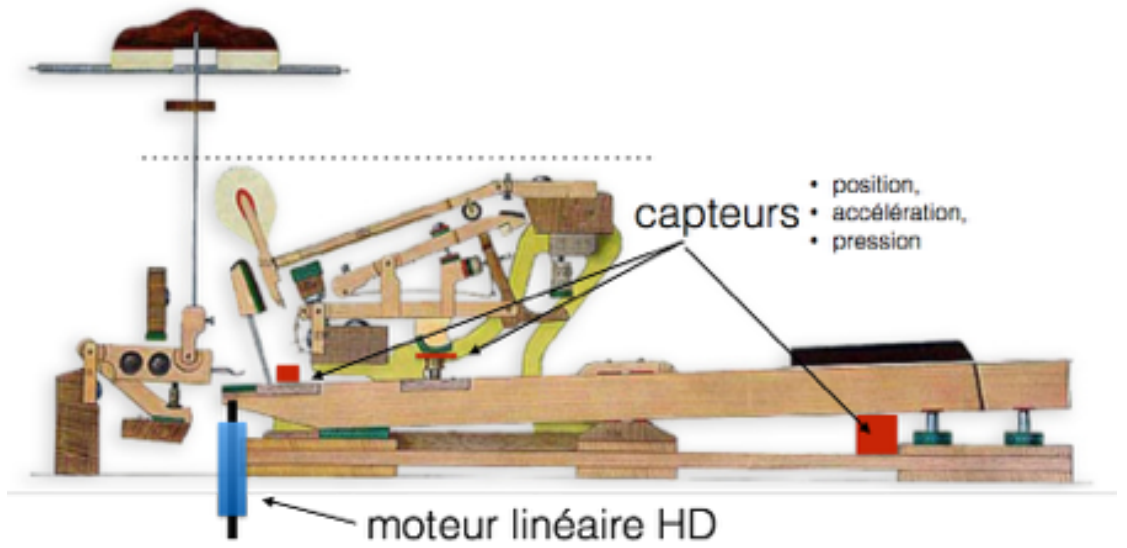
\includegraphics[width=15cm]{MECA_PIANO3.png}\hss}\hfill\null
   	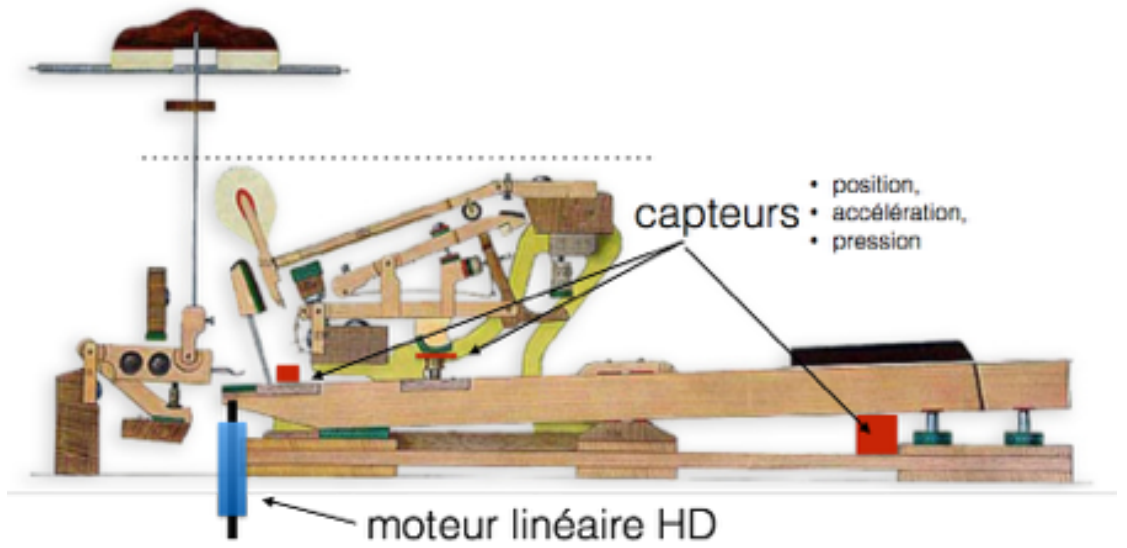
\includegraphics[width=15cm]{MECA_PIANO3.png}
 		\caption{Mécanique de type Renner avec un modèle 3D de l’actuateur linéaire}
	\end{figure}

%Figure 3: une implémentation possible du moteur et des capteurs. Plusieurs types de
%capteurs sont envisageables, accéléromètre sur la touche, capteur de pression entre la
%touche et le pilote, capteur de position sous la touche. Nous étudierons les propriétés de
%chacun et adopterons celui ou la combinaison de ceux qui donnent le meilleur rendu par
%rapport au touché original.

Pour guider les idées, un schéma envisageable d’implémentation est proposé sur la figure 3. L’implémentation optimale nécessite bien-sûr une étude plus approfondie, il s’agit simplement ici de se de fixer les idées. Le moteur et les capteurs de positions sont représentés par les rectangles bleus ou rouges. Sur cette proposition, le rapport (R) entre l’action du moteur et celui du marteau est le même que pour le doigt de l’artiste soit environ 5,5. Les modifications apportées à la mécanique originale sont minimales. Avec un réglage approprié, la sensation
de toucher sera adaptable aux désirs de l’artiste et restera très proche des sensations offertes par la mécanique à répétition et ce même si les marteaux sont lourds car le moteur accompagne en le soutenant le mouvement de la touche mais ne s’y substitue pas totalement.

  \section{Boucle d'asservissement}

La qualité de la boucle de feedback est un point essentiel de notre entreprise. C’est ici que l’expertise de Laurent Bessières donne tout son sens musical au projet. L’asservissement devra d’une part donner aux artistes un confort de jeu digne des meilleures mécaniques avec en plus un équilibrage parfait sur toute l’étendue du clavier. D’autre part, et c’est peut être le plus important, un certain nombre de paramètres de la boucle d’asservissement seront modifiables.

L’échappement et la façon dont il se déroule constituent l’épicentre de l’expressivité. Nous en avons bien conscience et notre intention est bien de le conserver tel quel afin que l’artiste ne soit pas perturbé et puisse donner le meilleur de lui même. Le résultat final dépend également d’un mariage harmonieux entre la mécanique/clavier et l’ensemble harmonique et nous devrons procéder par étape. D’abord assurer que l’apport d’énergie peut se faire de manière quasi transparente pour l’artiste, ensuite exploiter les possibilités offertes par cet apport. Deux axes seront explorés en priorité :

\begin{itemize}
\item  le paramétrage de la courbe de réponse de la mécanique en fonction de l’énergie fournie par l’artiste. On peut élargir ou rétrécir la gamme dynamique et rendre la courbe de réponse non linéaire et des degrés aussi divers qu'imaginables.

\item  la modification physique des éléments de la mécanique, comme le poids et les têtes de marteaux et, en allant plus loin, le point de frappe.
\end{itemize}

Sur tous ces domaines, l’expertise de Laurent Bessières est fondamentale aussi bien pour identifier les paramètres de contrôle que pour qualifier leur gamme et pour la bonne intégration de l’ensemble dans l’instrument. La programmation des fonctionnalités dans le FPGA qui calculera les commandes du moteur à partir des données des capteurs sera elle réalisée par les ingénieurs du LPNHE.

\newpage

  \section{Modélisation}

Thomas Hélie, chercheur à l’IRCAM au Laboratoire des Sciences et Technologies de la Musique et du Son, est spécialiste de la modélisation physique d’instruments de musique. L’un de ses projets de recherche concerne notamment la modélisation, l’asservissement et la commande d’une bouche artificielle robotisé pour le jeux de cuivre. Dans le cadre de notre projet son expertise nous permettra de modéliser les performances de la boucle de feedback en fonction des paramètres mécaniques que nous pouvons ajuster (position de l’actuateur, nombre, nature et position des capteurs). Disposer d’un modèle nous permettra de choisir les configurations les plus prometteuses avant de les réaliser plutôt que d’avoir à toutes les construire et toutes les essayer.

La méthode des systèmes Hamiltionien à ports (Port Hamiltonian System ou PHS) nous permettra de réaliser ces modèles. Cette approche où le système physique étudié est représenté par un ensemble de composants (éléments stockant de l’énergie, éléments dissipatifs, sources externes) reliés par des connexions conservatives (bilan d’énergie ou de puissance) permet une modélisation numérique relativement simple des systèmes complexes. Cette représentation garantie par ailleurs que les lois de conservations sont satisfaites à toutes les interfaces. La modularité du PHS permet d’envisager une complexité graduelle de la modélisation jusqu’à représenter de manière très réaliste l’ensemble touche, chevalet, marteaux ainsi que les commandes d’étouffoir et les ressort de rappel. Dans ce cadre nous nous appuierons également sur les travaux de Xavier Boutillon concernant la modélisation extrêmement réaliste du toucher des mécaniques de piano à queue.

Notons également que l’approche PHS permet d’étudier les réponses non linéaires aux actions extérieures et de calculer les (pré-)contraintes à appliquer sur le signal d’entrée pour obtenir la réponse souhaitée (platitude). Cette approche nous permettra alors de calculer avec précision les paramètres de la boucle d’asservissement. Là encore l’expertise de Thomas Hélie nous permettra d’élaborer ces modèles de manière efficace et optimale.



%--------------------------------------------------------------------------------------
%
% Caractérisation technique du projet
% objectifs
% déroulement prévu
%
%--------------------------------------------------------------------------------------
\part{Projet "CHAMP", étude et caractérisation}

	\chapter{Introduction au projet}
	
	\section{Synthèse et objectif du projet}
	
	Comme dis précédemment, le projet "CHAMP" est né de la rencontre de personne et de la mise en commun de savoir provenant d'univers varié, à savoir, 
	
	le milieu scientifique, au travers du LPNHE (laboratoire de physique nucléaire et des hautes énergies), représenté par Antoine LETESSIER SELVON, physicien des hautes énergies et directeur de recherche, Hervé LEBBOLO, ingénieurs de recherche, et enfin,  Philippe REPAIN, mécanicien chef d'atelier.
	
	le milieu musical artisanal, représenté par Laurent Bessières détenteur du prestigieux titre d'Académicien Steinway.
	De plus, depuis l'inauguration de la philharmonie de Paris en janvier 2015, Laurent en est l'accordeur référant de la philharmonie. Enfin, il travaille également avec d'autres prestigieuses salles, comme Steinway and Sons France, régie Pianos, la Salle Pleyel, la Salle Cortot ou le Studio de la grande Armée qui font régulièrement appel à ses services.	
	
	Au travers de cette rencontre, plus que de vouloir proposer un piano de concert connecté, nouvelle génération, le projet prend racine au travers d'une idée simple mais précise, élargir les possibilités de l'instrument en n'en modifiant la mécanique interne, tout en conservant inchangé, l'expérience utilisateur.
	Pour cela, décision fut prise de s'appuyer sur les techniques et les technologies modernes afin de faire évoluer l'instrument, le piano.
	
	Ainsi, sans altérer l'expérience utilisateur, ce rapport étroit entre le musicien et son l'instrument, représentant de nombreuses années de pratique, les artistes auront à disposition des nouveaux moyens d'expression, offrant de nouvelles possibilités de jeux.
	
	\newpage
	
		\subsection{Un nouveau moyen d'expression}
		
		Afin de proposer de nouveaux moyens d'expression, il a tout d'abord fallu identitfier au sein du piano, l'élément étant la source de l'identité "musicale" ; des harmoniques de l'instrument. C'est en modifiant, en retravaillant la mécanique autour de cette pièce, que nous pourrons apporter de nouvelles expériences de jeux.
		
		Grâce aux articles de spécialistes, précédemment cité, le marteau, plus que la touche ou le chevalet, apparaît comme éléments ayant l'incidence majeure sur l'harmonisation de l'instrument, au travers de son poids.
		
		L'intégration de nouvelles technologies au sein du projet, aura donc pour but de permettre une variation du poid du marteau, afin de fournir une large palette d'harmonique au musicien, qui n'aura plus qu'à laissé court à son imagination et à sa technique afin de tiret le meilleur de l'instrument lors de composition musicale.
	
	\section{Rôle au sein du projet}	
	
	Recruté en tant que stagiaire, assistant ingénieurs, sur ce projet. Mon rôle fut prendre connaissance du projet, étudier l'état de l'art quant aux recherches déjà effectué et d'avoir un regard critique sur ces dernières. Être force de propositions sur l'intégration de solutions techniques, sur des problématiques direct, ainsi que sur des fonctionnalités futur; les développer et enfin mener leurs intégrations au sein du projet.
	
	Avant mon arrivée, l'équipe en place avait déjà commencé à travailler sur une preuve de concept, s'appuyant sur une base d'électronique analogique, cœur de métier du laboratoire. Mais suite à mon arrivée, nous avons ensemble, redéfini le cadre du projet, afin de garder les idées et concepts testés et approuvés lors cette première approche, tout en faisant évoluer le projet en basculant sur une base orientée électronique numérique, système embarqué.
	
	De plus, j'ai eu pour rôle de faire part de l'avancement de mon travail, ainsi que mes observations autour du projet, à mon maitre de stage et directeur de recherche, lors de réunion durant lesquels nous définissions ensemble l'avancement des différentes étapes et discutions de nouvelle(s) fonctionnalité(s) pouvant être intégré au projet.
	
	Enfin, j'ai pu être force de proposition quant aux futur fonctionnalité du projet, ce derniers étant une preuve de faisabilité, il dispose d'un cahier des charges au contour assez vague, induisant une plus grande liberté d'esprit, quant aux innovations pouvant être apportées.	
	
	
	\chapter{Les travaux menés}
	
	Comme expliqué précédemment, suite à mon arrivé au LPNHE, j'ai commencer par prendre connaissance de l'architecture globale du projet (figure ci-dessous) et des concepts et idées qui avaient déjà étés pensé et proposé, ainsi que des diverses solutions techniques à l'étude concernant des choix de composants.
	
	J'ai ainsi commencer par travailler sur le développement de la chaine de contrôle la plus simple pouvant être mise en place, afin d'éprouver les choix et solutions techniques retenu.
	Cette chaine, représentant l'action d'une touche du piano, ce comporte comme suivant: Un accéléromètre mesurant l'accélération du marteau, (du à une force appliqué sur une touche du piano) communiquant avec une carte programmable munie d'un FPGA, appliquant un filtre numérique sur les données reçu, pour ensuite les faire parvenir à un convertisseur numérique analogique (CAN), assurant la transmission des données à notre contrôleur moteur.\newline
	
	\begin{figure}[!ht]
    \center
    %\hfill\hbox to 0pt{\hss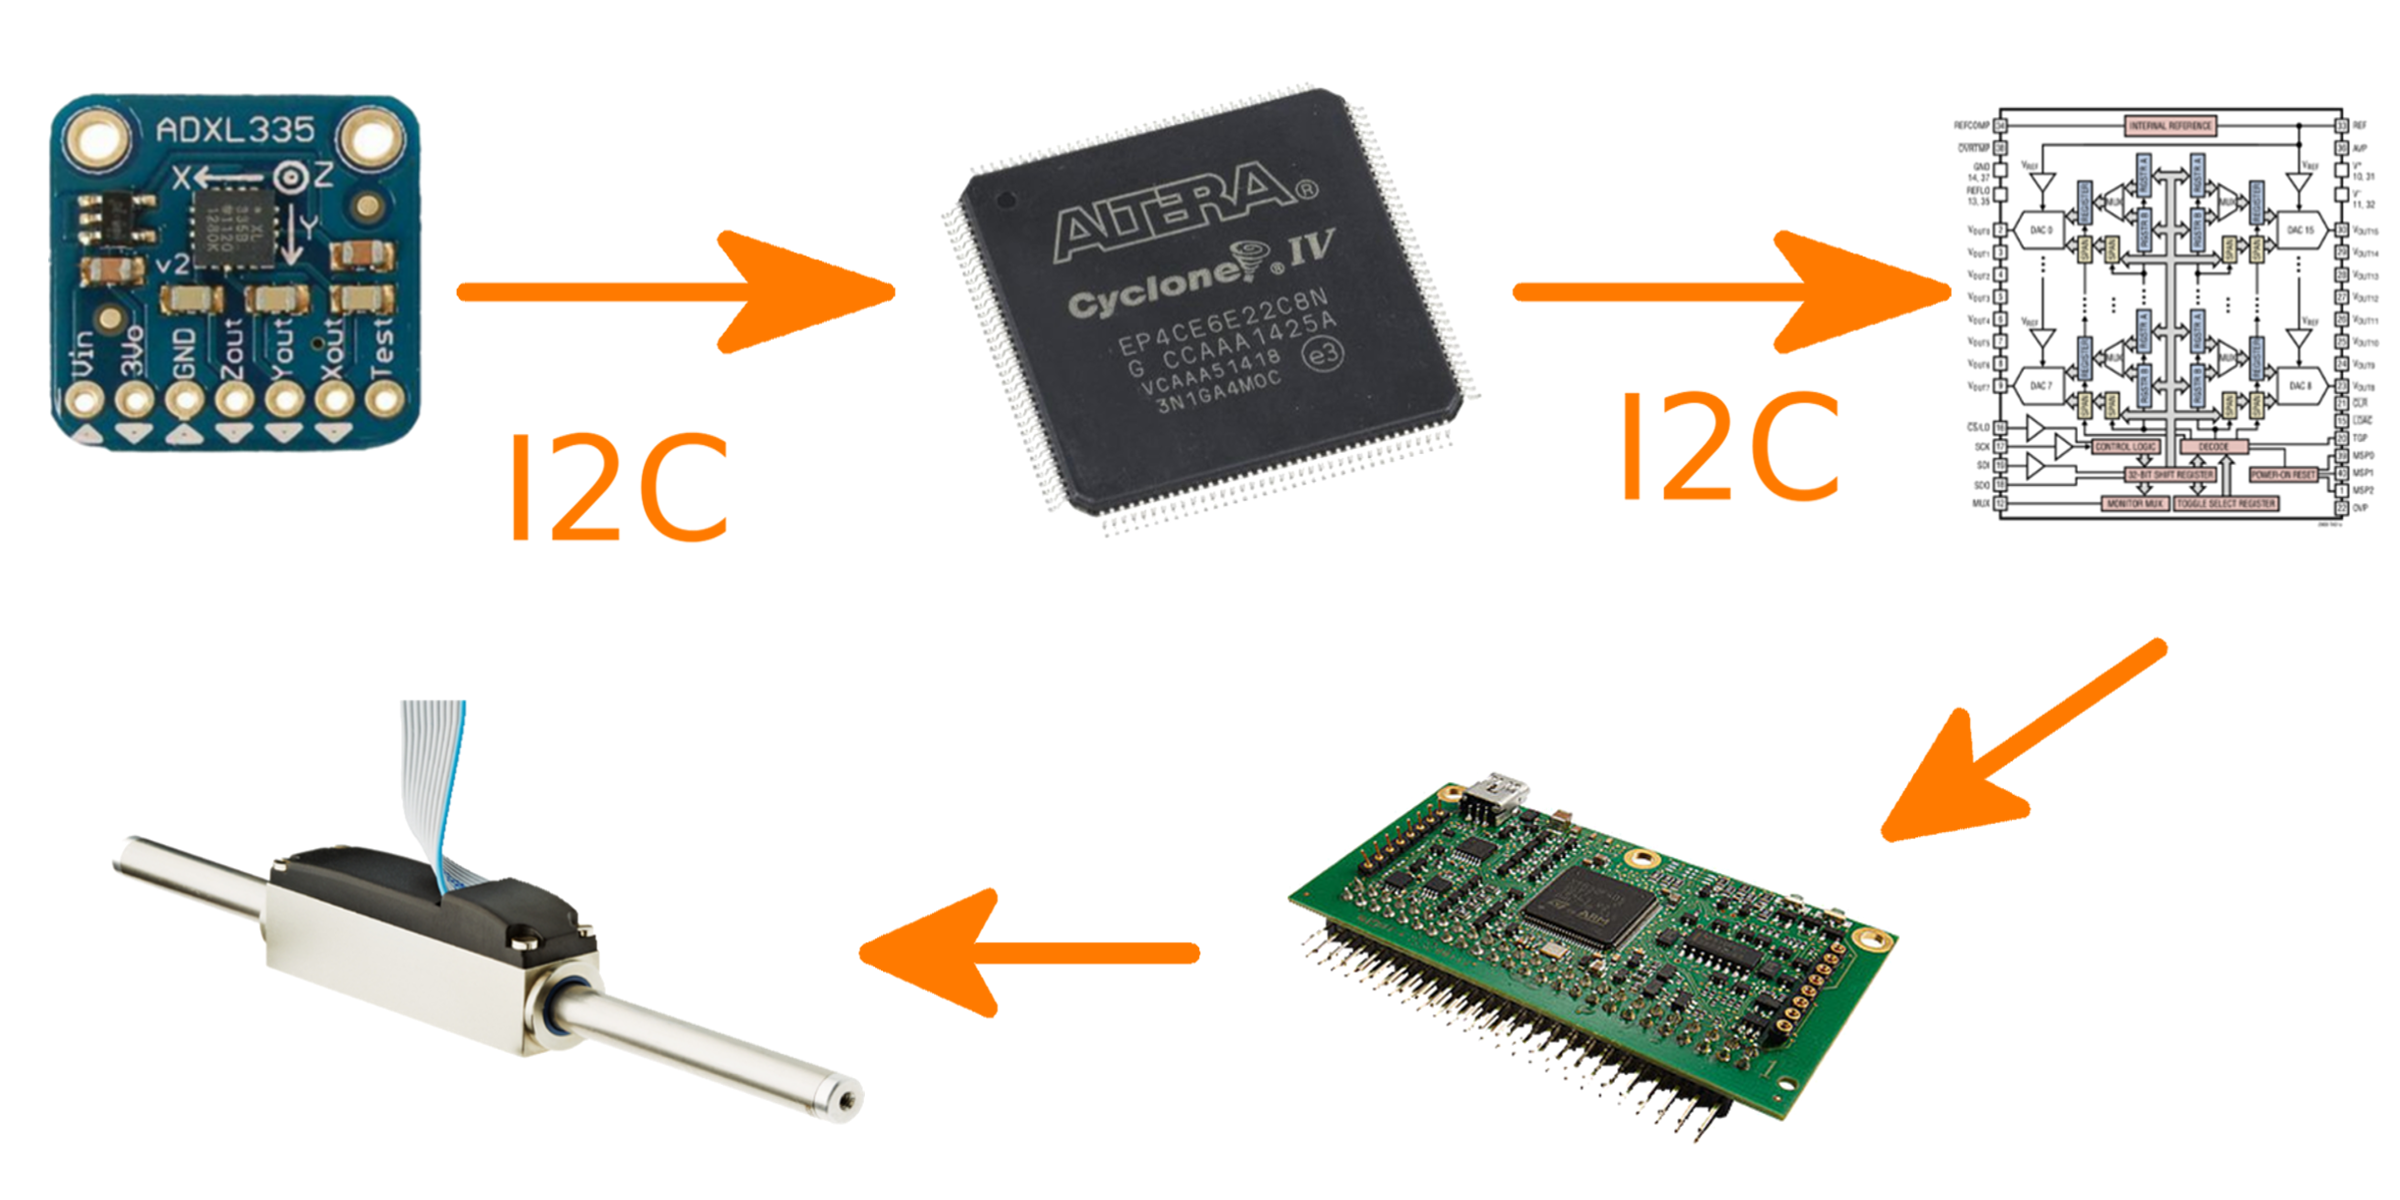
\includegraphics[width=17cm]{CH.png}\hss}\hfill\null
  	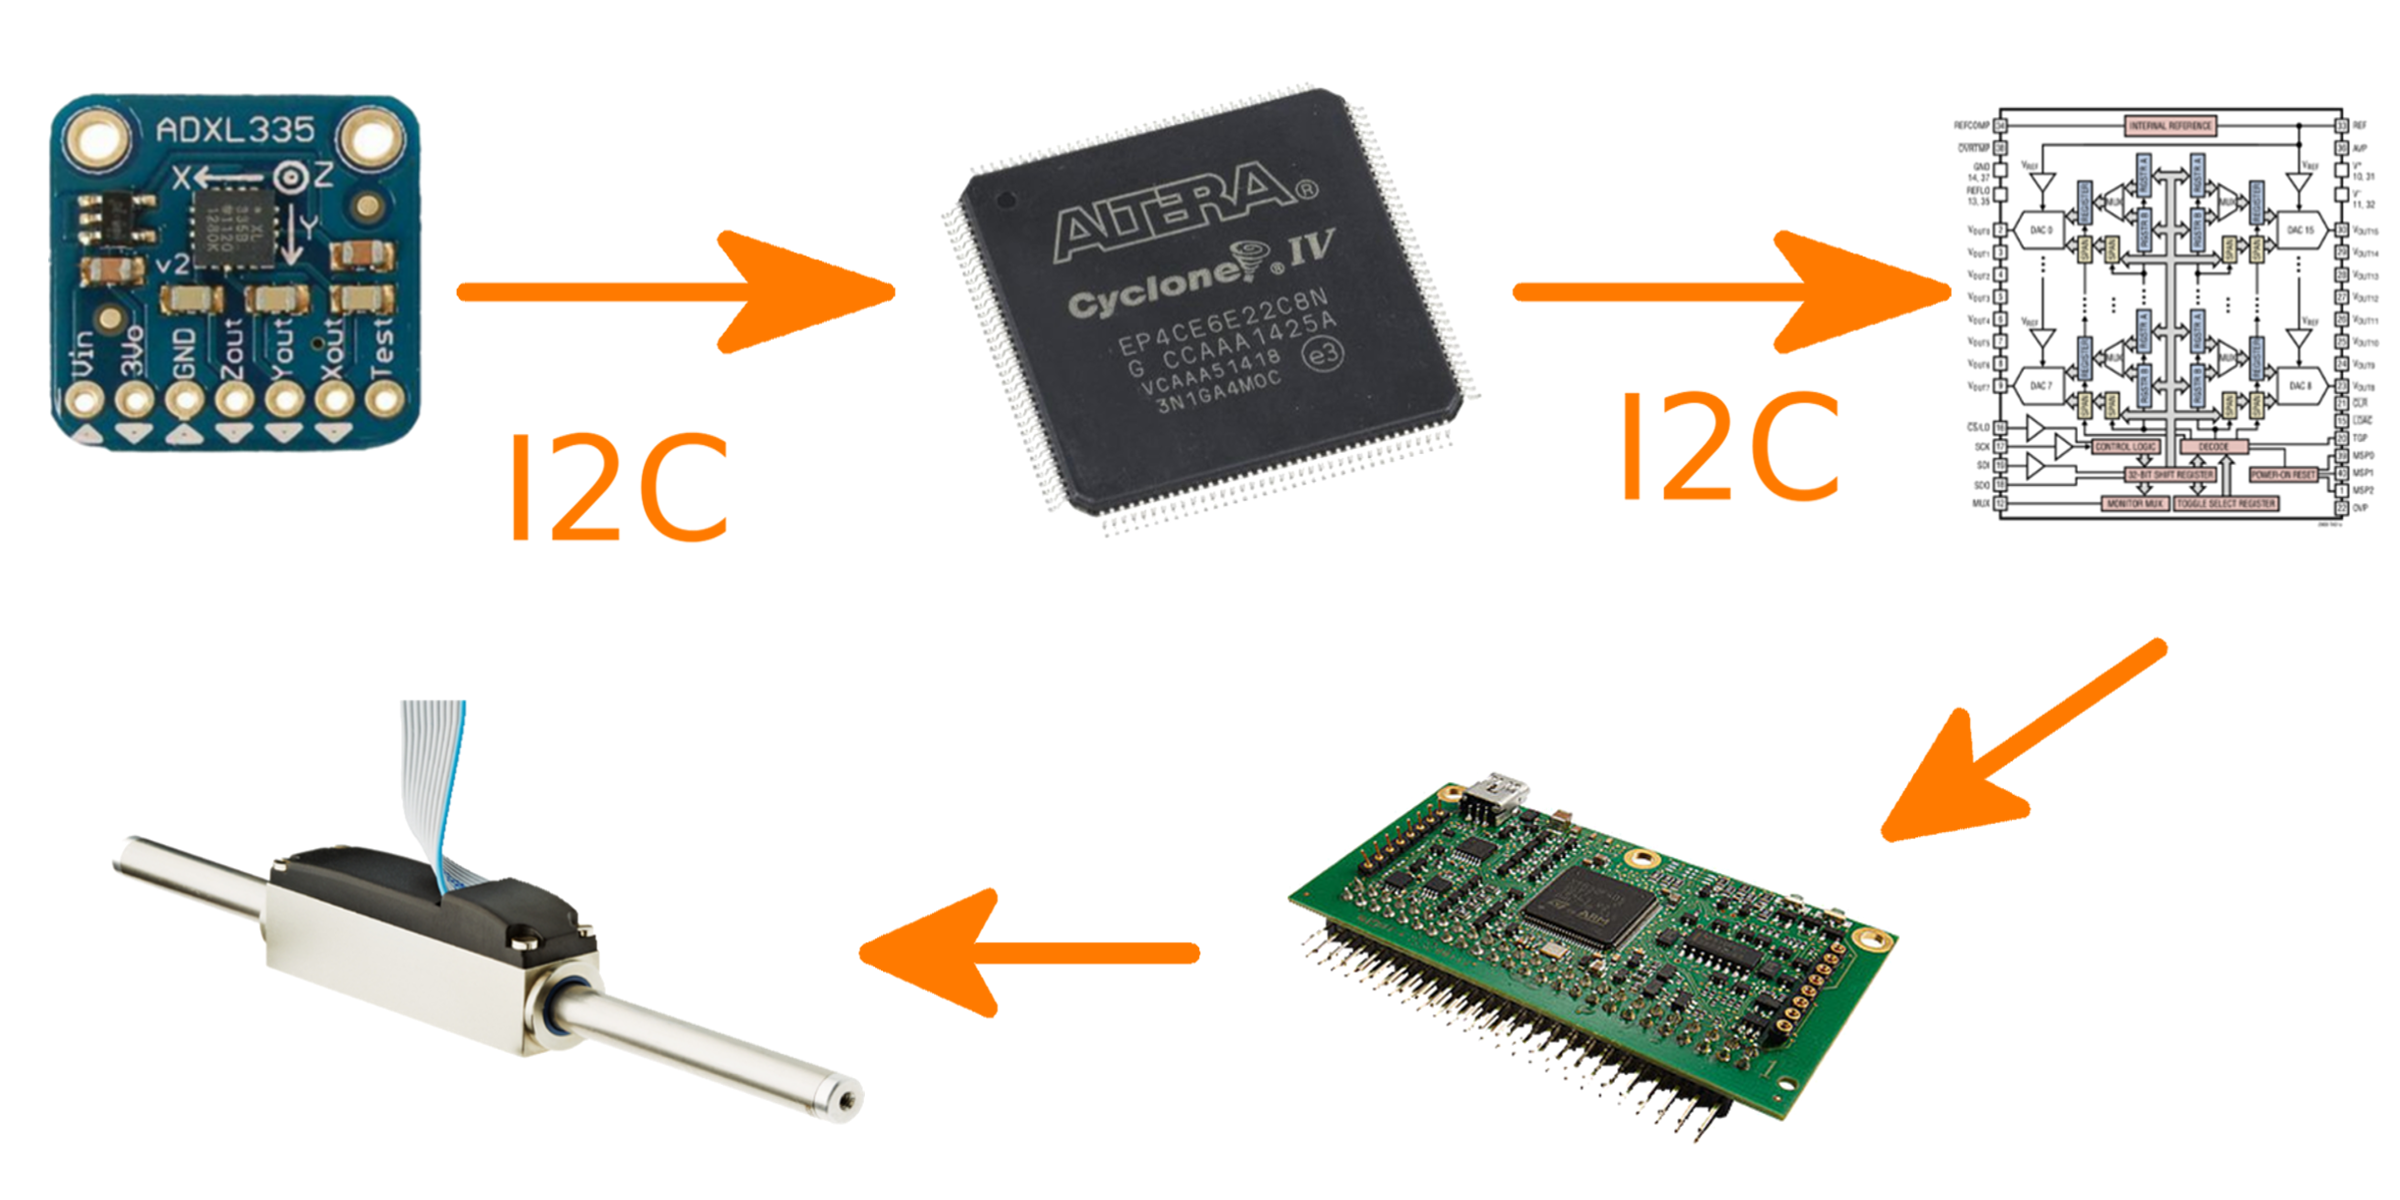
\includegraphics[width=17cm]{CH.png}
    \caption{Chaine de contôle d'une touche de Piano}
	\end{figure}	
	
	Ainsi, la toute première tâche réalisé fut de mener une étude de cas entre les deux bus de communication à disposition, le bus I2C et le bus SPI, afin de déterminer lequel serai le plus adapter à notre projet.
	
	Cette étude de cas, m'a par la suite conduit à éprouver un "hacking" sur notre accéléromètre. Notre choix de bus de communication induisant un grand notre de câble de branchement, nous souhaitions en faire diminuer le nombre.
	
	La suite logique à cette étape, fut d'étudier le bus de communication sélectionné, afin de l'instancier au sein du projet, en ce basant sur le langage VHDL. Ce bus de communication étant présent en deux endroit de la chaine, entre l'accéléromètre et la carte programmable FPGA et entre cette dernière et notre convertisseur numérique analogique, notre intégration devais répondre aux spécificités des deux cas d'utilisations, afin de ne pas faire doublons dans la mise en place de solution, ainsi que dans les potentiels sources d'erreurs.
	
	Puis, après avoir éprouver l'échange de données, entre les différentes entités, un filtrage numérique fut intégré à notre carte programmable. Ce filtrage ayant pour but de mettre en place un asservissement numérique sur le contrôle des moteur.
	
%	Par la suite, nous avons choisi de mettre en place une solution de monitoring, afin de pouvoir visualiser nos données échangés ,en temps réel sur un ordinateur.

	Par la suite, différents prototypes de cartes électronique (PCB) on du être réaliser et réévalué au long su projet, afin de répondre aux impératifs d'intégration matériel au sein du piano.
	
	Enfin, une étude de "rétro-engineering", fut mené en salle de teste sur des éléments électroniques tiers, fournie par notre partenaire technique, l'entreprise "Faulhaber", afin d'en vérifier le bon fonctionnement, mais également d'en valider le comportement vis-à-vis de l'utilisation souhaité.
	
	Mais comme expliqué en ce début de partie, ce module, illustré ci-dessus, n'est que 1/12 ème du prototype final; ne permettant la récupération et le traitement que d'un seul accéléromètre à la fois et donc, d'une seul touche à la fois.
	
	La maquette à réaliser étant composé de 12 touches, il nous faudra par la suite, généraliser notre module afin de récupérer et traiter les informations de nos 12 touches, de manière parallèle.
	Ce travail étant un peu plus complexe que le module précédemment présenté, il demande une refonte d'une partie de la chaine, vis-à-vis de l'échange de données entre la carte programmable (FPGA) et le convertisseur numérique analogique (CNA).
	
	\chapter{Planning}

	Ci-dessous sont présenté sous forme de diagramme de Gant, le calendrier prévisionnel ainsi que le calendrier réel du travail réalisé tout au long su stage.
	On y retrouve un descriptif complet et détaillé des différentes tâches réalisés.
	
	On peut observer sur le calendrier réel, que les phases de test, de débug, n'avait pas été prise en compte lors de l'établissement du calendrier prévisionnel.
	A l'avenir, ces tâches ne seront plus négligé, étant donné le caractère important de celles-ci, du fait de leurs capacité à bloquer l'avancement d'un projet, et induire des retards plus ou moins important.
	
	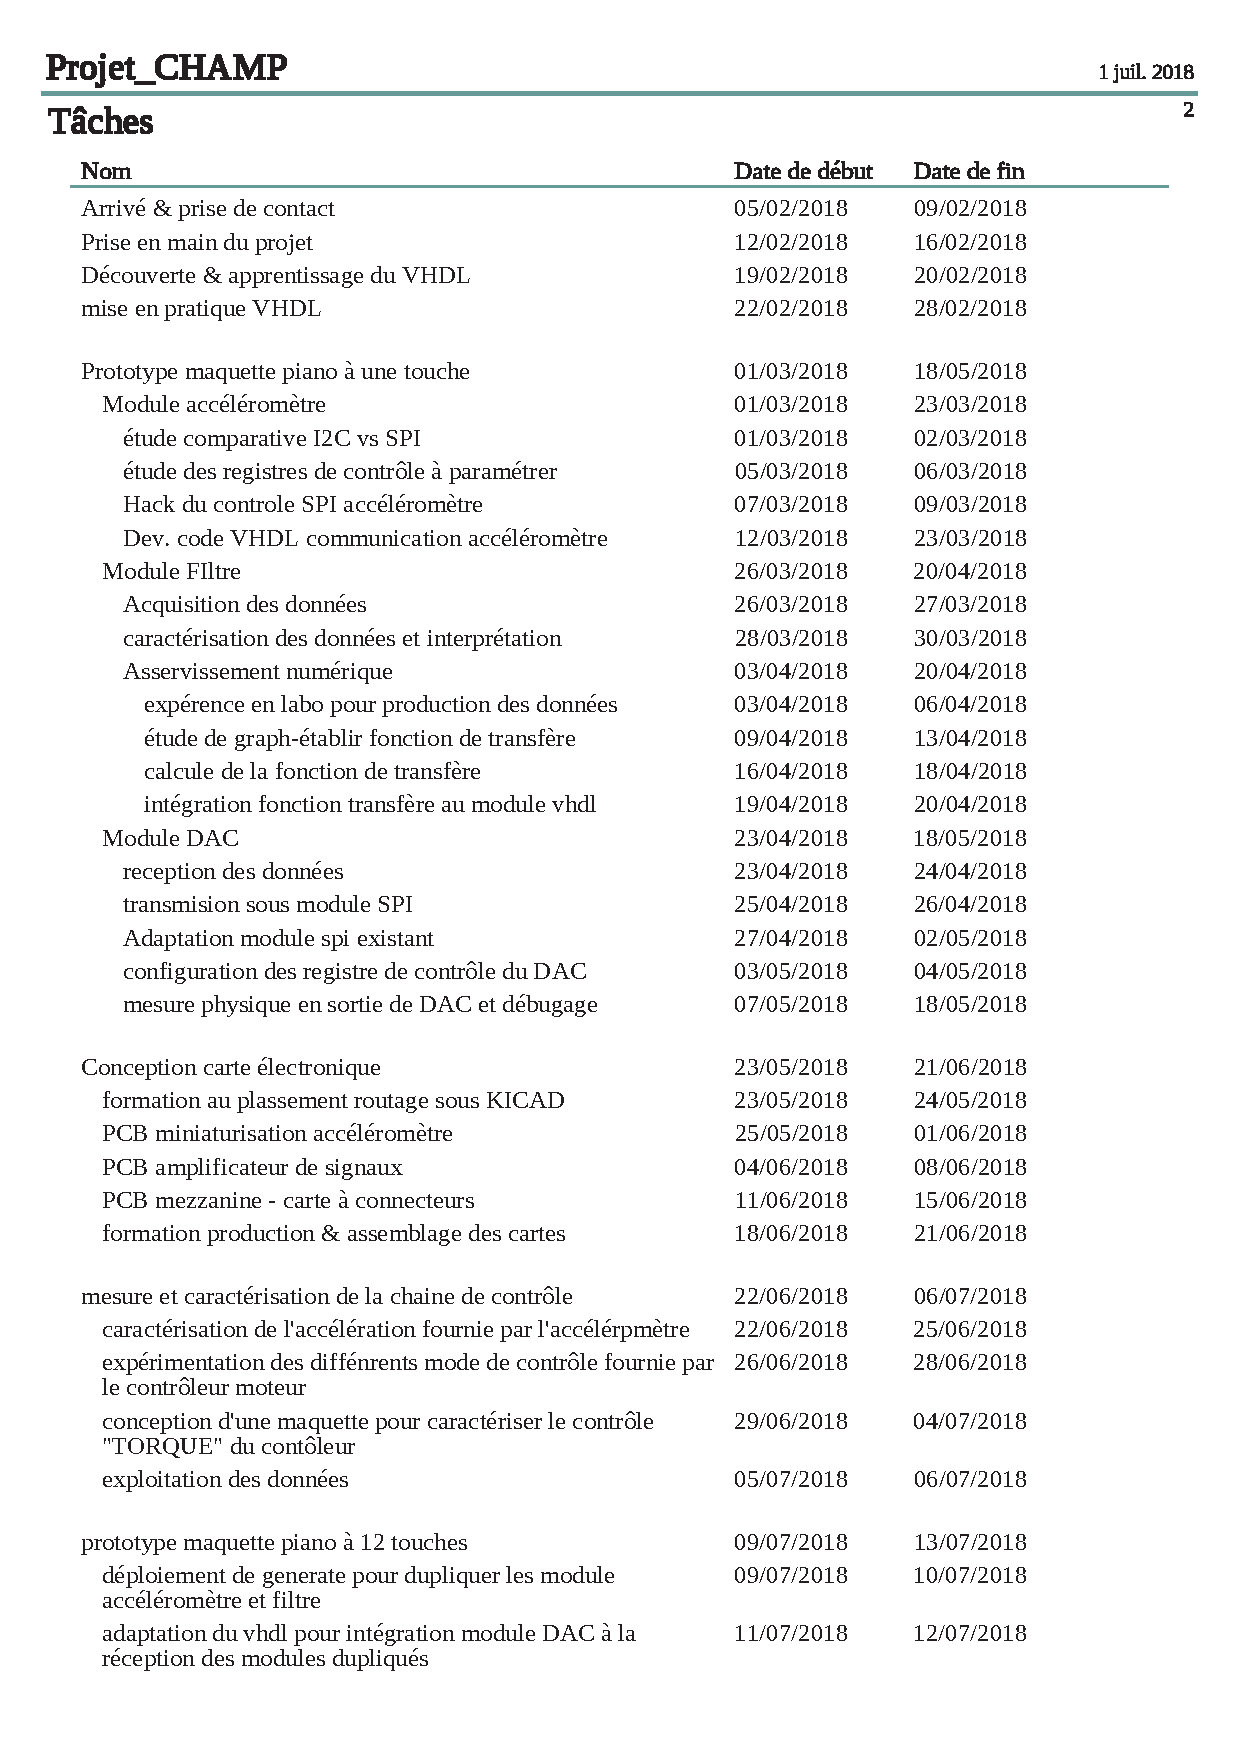
\includepdf[scale=1, pages=-]{calendrier_Previsionnel_defA}
	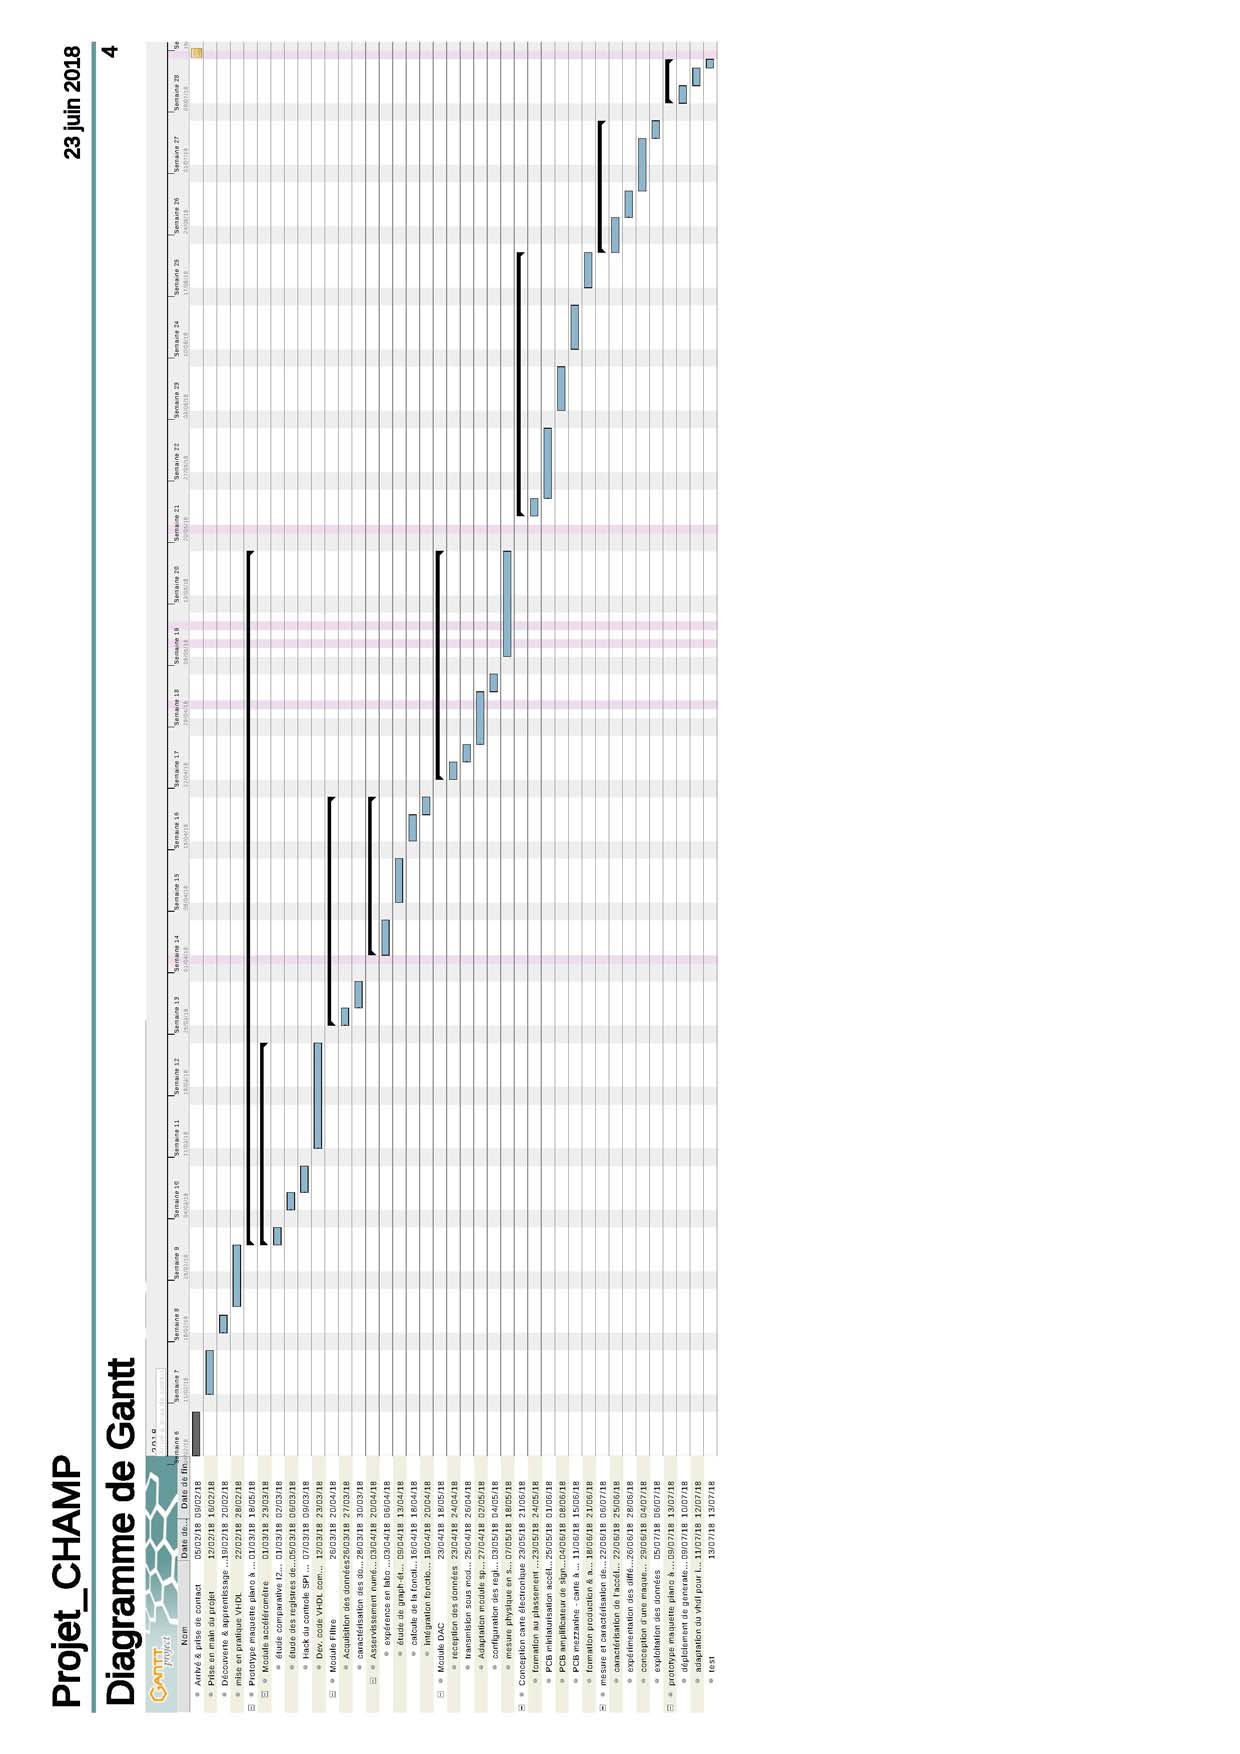
\includepdf[scale=1, pages=-]{calendrier_Previsionnel_defB}
	
	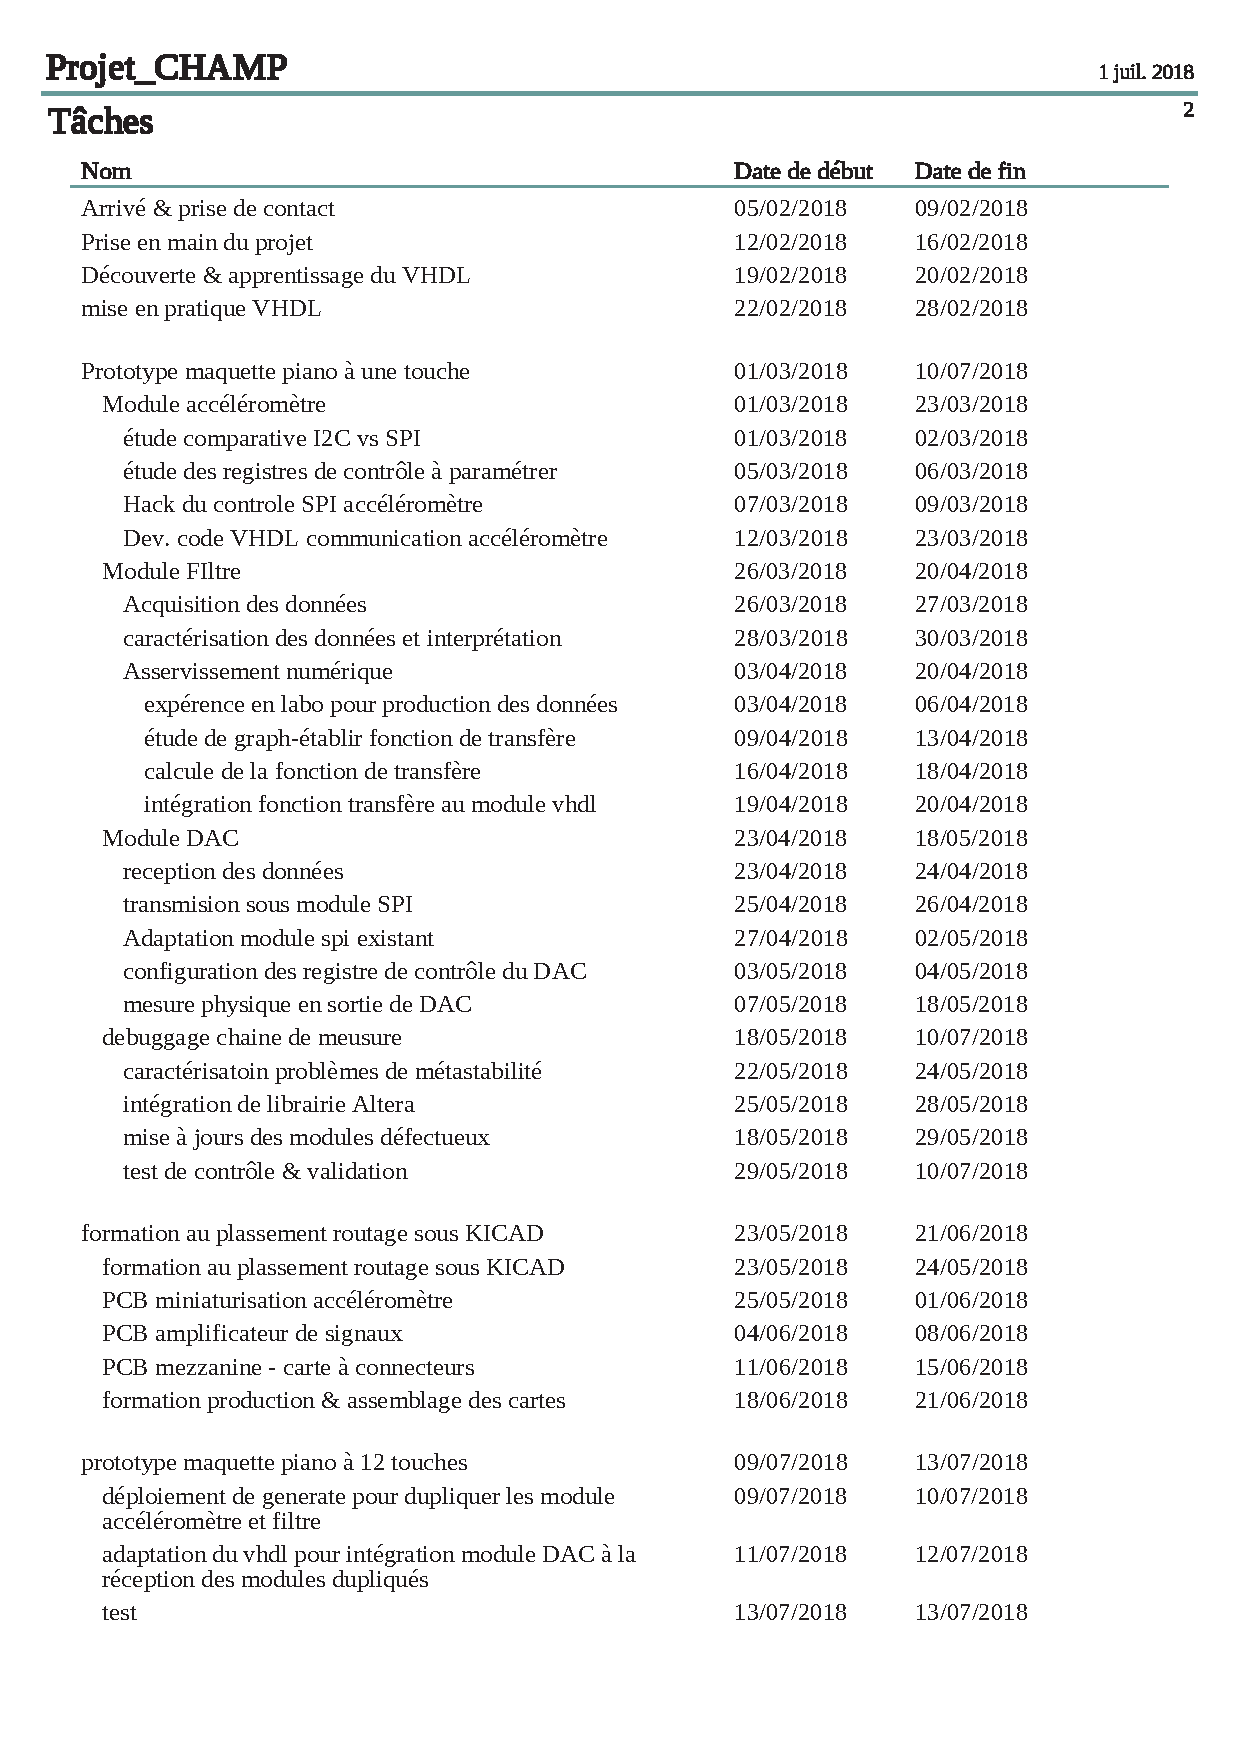
\includepdf[scale=1, pages=-]{calendrier_reel_defA}
	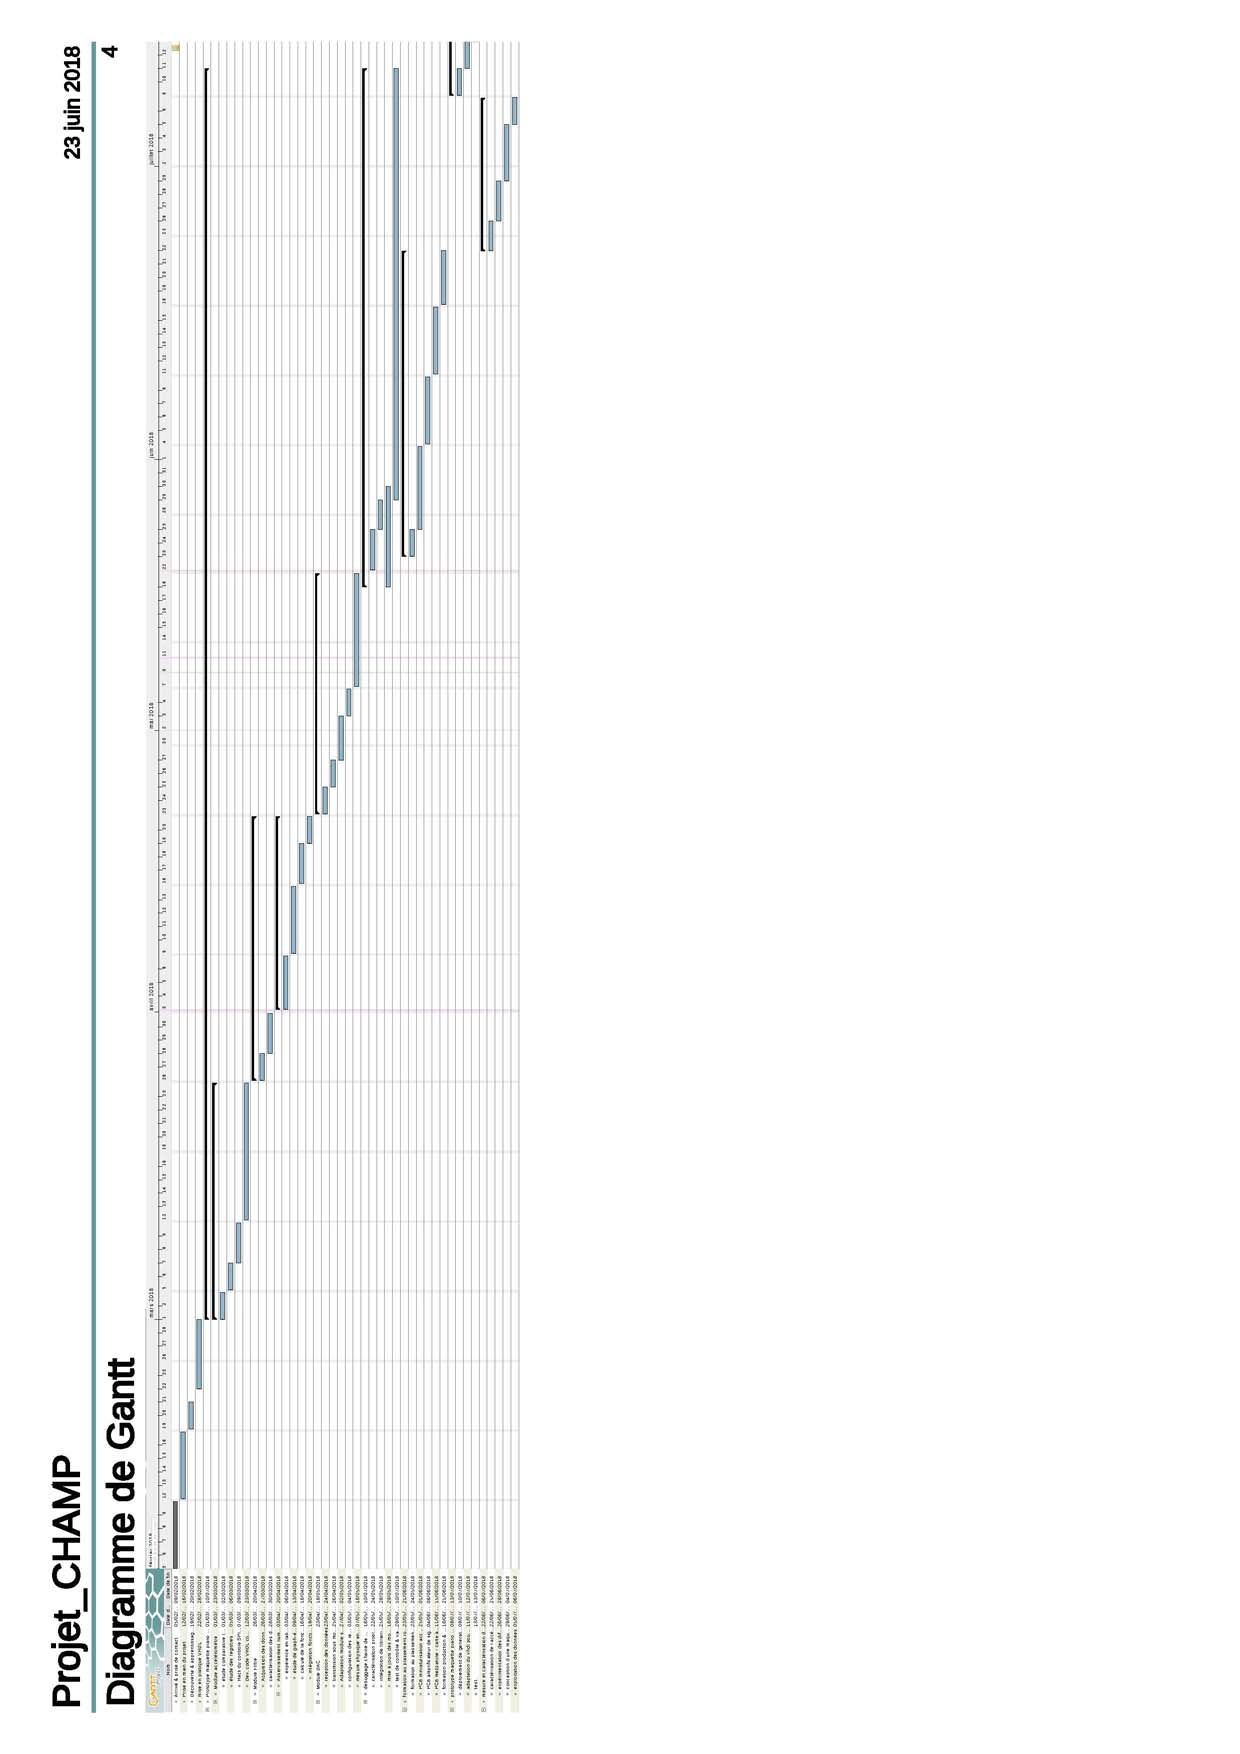
\includepdf[scale=1, pages=-]{calendrier_reel_defB}	
	
	
	
	
%--------------------------------------------------------------------------------------
%
%	Présentation et Détail des travaux Réalisés durant le stage
%
%--------------------------------------------------------------------------------------

	
	\part{Travaux et réalisation}	
	
	\chapter{Réalisation de la chaine de contôle}
	
	
	
	
	\chapter{Asservissement et caractérisation}
	
	Lors de la précédente partie, nous avons abordé l'ensemble des aspects qui nous ont permis de mettre au point notre chaine de contrôle; en partant des données fournies par notre accéléromètre, leurs réceptions et leurs traitement au sein de notre carte programmable (FPGA), jusqu'à leurs envoie et leurs réception par le Convertisseur Numérique Analogique, permettant le contrôle du contrôleur moteur, en lui transmettant des consignes de fonctionnement.
	
	Lors de cette partie, nous allons nous concentrer sur la mise au point de l'asservissement numérique, élément indispensable, devant prendre place au sein du filtre numérique de notre carte programmable FPGA.
	
	L'asservissement numérique est un procésus en plusieurs étape, consistant à piloter un système tiers, en mesurant périodiquement des valeurs de consigne, fournie par un système de capteurs, dans notre cas, un accélérommètre. 
	Par la suite, ces données sont traité par notre calculateur, mais étant donné le mode de traitement des inforamtions imposé par notre calculateur est de nature numérique et cadensé dans le temps de façon périodique grâce à une horloge; les informations en entrée, provenant de nos capteurs, sont donc des grandeurs discrètes.
	
	Les différentes étapes que l'on retrouve,  générique à tout système asservie sont les suivantes:
	
	\begin{itemize}
		\item l'échantillonage d'un signal continu
			Cette opération consiste à relever les informations prises par un signal continuà intervalles de temps
			régulier, appelée période d'échantillonnage. On parle alors de signal échantillonné, signigiant que le
			calculateur ne tiendra compte que des valeurs prises par le calculateur aux instants d'échantillonnage.
			
		\item La conversion d'un signal analogique en un signal numérique
			Il s'agit de convertir la valeur prise par un signal analogique à l'instant d'échantillonnage en une
			valeur numériqu,e afin qu'elle puisse être traitée par le calculateur. Un tel signal peut, par exemple, 
			provenir d'un capteur. On parlera alors de signal de mesure.
			 
		\item La conversion d'un signal numérique en un signal analogique
			Cette opération consiste à transformer le signal numérique issu du calculateur à l'instant 
			d'échantillonnage (on parlera de signal numérique de commande), en signal analogique de commande 
			existant sur toute la période d'échantillonnage, l'objectif étant de commander le système physique.
			
		\item  La synthèse d'un algorithme de calcul
			Il s'agit d'établir une loi d'évolution du signal de commande numérique en fonction des signaux de mesure
			et de référence, également numériques, afin de permettre au système asservi de satisfaire un cahier des
			charges. Cette fonction est appelée correcteur numérique ou encore loi de commande numérique. Elle a pour
			objectif de déterminer la valeur du signal numérique de commande à un instant d'échantillonnage, à partir 
			d'un algorythme de commande, de mesure et de référence.
	\end{itemize}
	
	Ainsi, l'on peut résumer sous forme de schéma bloque une structure classique d'asservissement numérique comme suivant:
	
	\begin{figure}[!ht]
    \center
    %\hfill\hbox to 0pt{\hss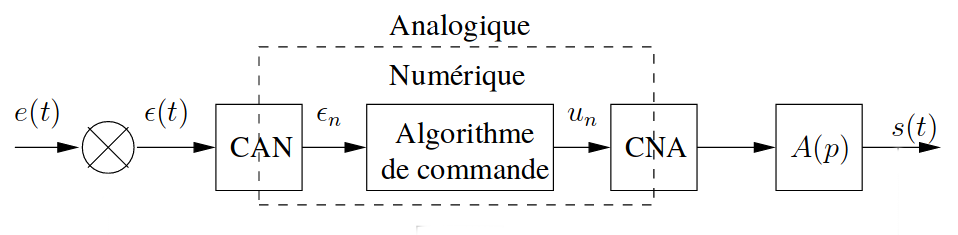
\includegraphics[width=17cm]{Assert_1.png}\hss}\hfill\null
  	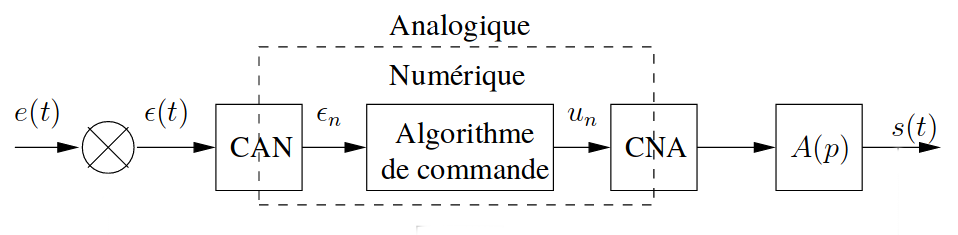
\includegraphics[width=17cm]{Assert_1.png}
    \caption{Structure classique d'asservissement numérique}
	\end{figure}	
	
	De plus, l'asservissement numérique de notre projet implique la caractérisation de la fonction de transfère de notre système dans son ensemble.
	Ainsi, afin de déterminer notre fonction de transfère, seront présenté les différents protocols et les différentes manipulations effectués sur notre banc de test.

	\section{Asservissement du projet Champ}
	
		Au sein de notre projet, notre asservissement va reprendre les différentes étapes présentés ci-dessus.
		
		Ainsi, concernant l'échantillonage d'un signal continu, cette étape est réalisé au sein de notre accéléromètre étant
		donné que ce dernier nous fournie un signal échantilloné à une fréquence de 1 KHz (Période de une millis seconde).
		Notre accéléromètre disposant d'un convertisseur analogique numérique intégré sur chaque axe, c'est au sein de ce
		derniers que s'effectue l'opération d'échantillonage du signal continue.
		
		Par la suite, c'est au sein de notre carte programmable FPGA que s'effectue la phase de traitement sur notre signal
		discret. C'est au sein de notre filtre numérique que va être appliqué l'algorythme de synthèse sur les mesures en
		provenance de l'accéléromètre, afin d'asservire le système contrôlé, selon le cahier des charges.
		
		Enfin, la fonction de conversion de notre signal numérique en un signal analogique est assuré par le convertisseur
		numérique analogique (CNA) ayant pour rôle de fournie une commande au conrôleur moteur, existant sur toute la période
		d'échantillonage, afin de commander notre système physique.
		
		Comme précédement, on peut résumé l'asservissement mise en place pour le projet CHAMP, sous la forme d'un shéma bloque, comme suivant:
		
	\begin{figure}[!ht]
    \center
    %\hfill\hbox to 0pt{\hss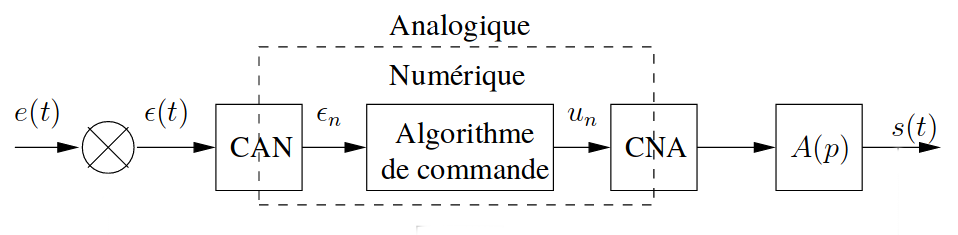
\includegraphics[width=17cm]{Assert_1.png}\hss}\hfill\null
  	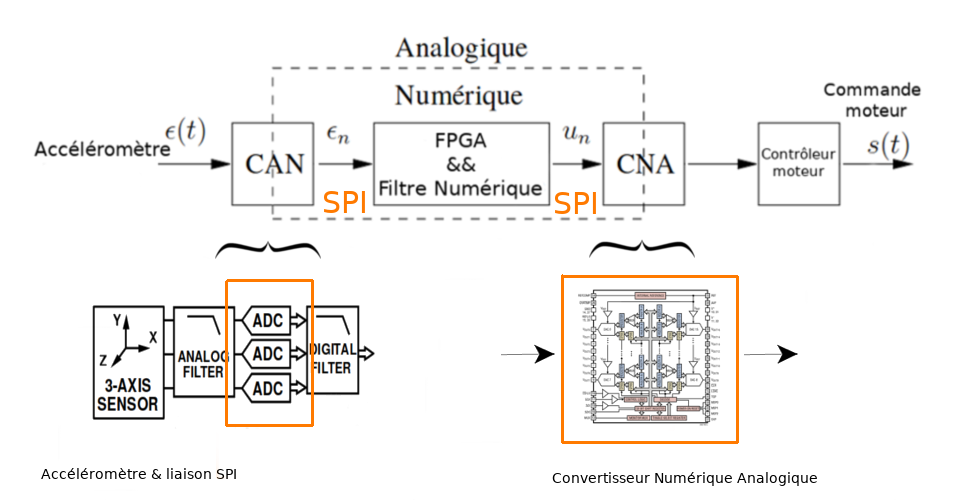
\includegraphics[width=17cm]{Assert_2.png}
    \caption{Asservissement numérique du projet CHAMP}
	\end{figure}	
		
		
	\section{Fonction de transfère}
	
		La fonction de transfère de notre système correspond à l'algorythme, appliqué sur nos données (discrètes) au sein du filtre. Une fois les données sortie de cet algorythme, les données sont haptes à piloter notre système tiers comme nous le souhaitons.
		
		Une fonction de transfère est le modèle mathématique de la relation entre la sortie et l'entré de notre système ; le plus souvent cette fonction étant invariante en fonction des paramètres d'entrés.
		Du point de vue d'une approche physique, la fonction de transfère caractérise la dynamique du système; elle ne dépend que de ses caractéristiques physique. 
		Ainsi, un système sera décrit par sa fonction de tranfert est représenté comme suivant:

	\begin{figure}[!ht]
    \center
    %\hfill\hbox to 0pt{\hss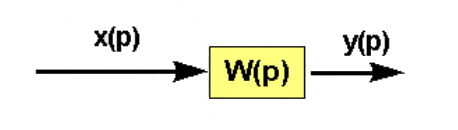
\includegraphics[width=17cm]{transf1.png}\hss}\hfill\null
  	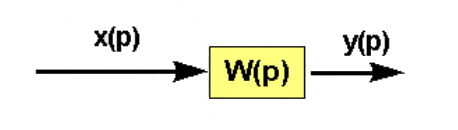
\includegraphics[width=5cm]{transf1.png}
    \caption{Modèle quelquonque}
	\end{figure}
	
	Nous aurons donc la fonction de transfère suivante : W(p) = Y(p) / x(p).
	
	\newpage
	
	\subsection{Première manipulation}
	
		A travers cette première manipulation, nous avons cherché à déterminer la fonction de transfère de notre modèle, comme le décris le shéma ci-dessous.
		
	\begin{figure}[!ht]
    \center
    %\hfill\hbox to 0pt{\hss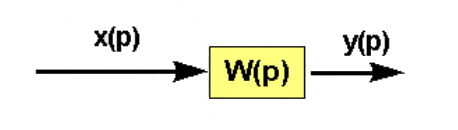
\includegraphics[width=17cm]{transf1.png}\hss}\hfill\null
  	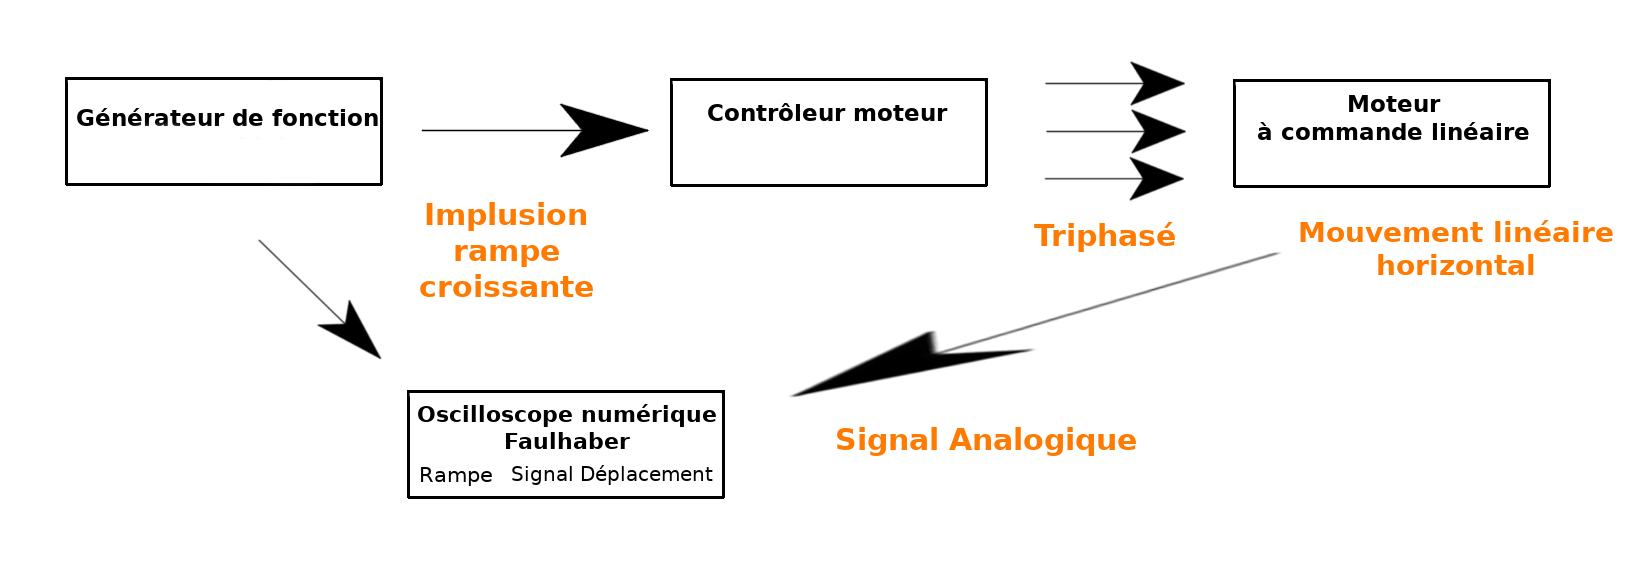
\includegraphics[width=18cm]{manip1.png}
    \caption{Schéma bloc - Première manipulation}
	\end{figure}	
		
		Nous avons utilisé un générateur de fonction 
	
	
	
	
	
	
	
	
	
	
	
	
	
	\subsection{Seconde manipulation}
	
		
		
	\begin{figure}[!ht]
    \center
    %\hfill\hbox to 0pt{\hss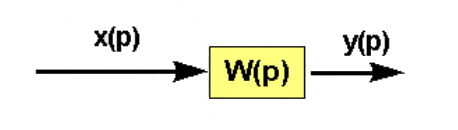
\includegraphics[width=17cm]{transf1.png}\hss}\hfill\null
  	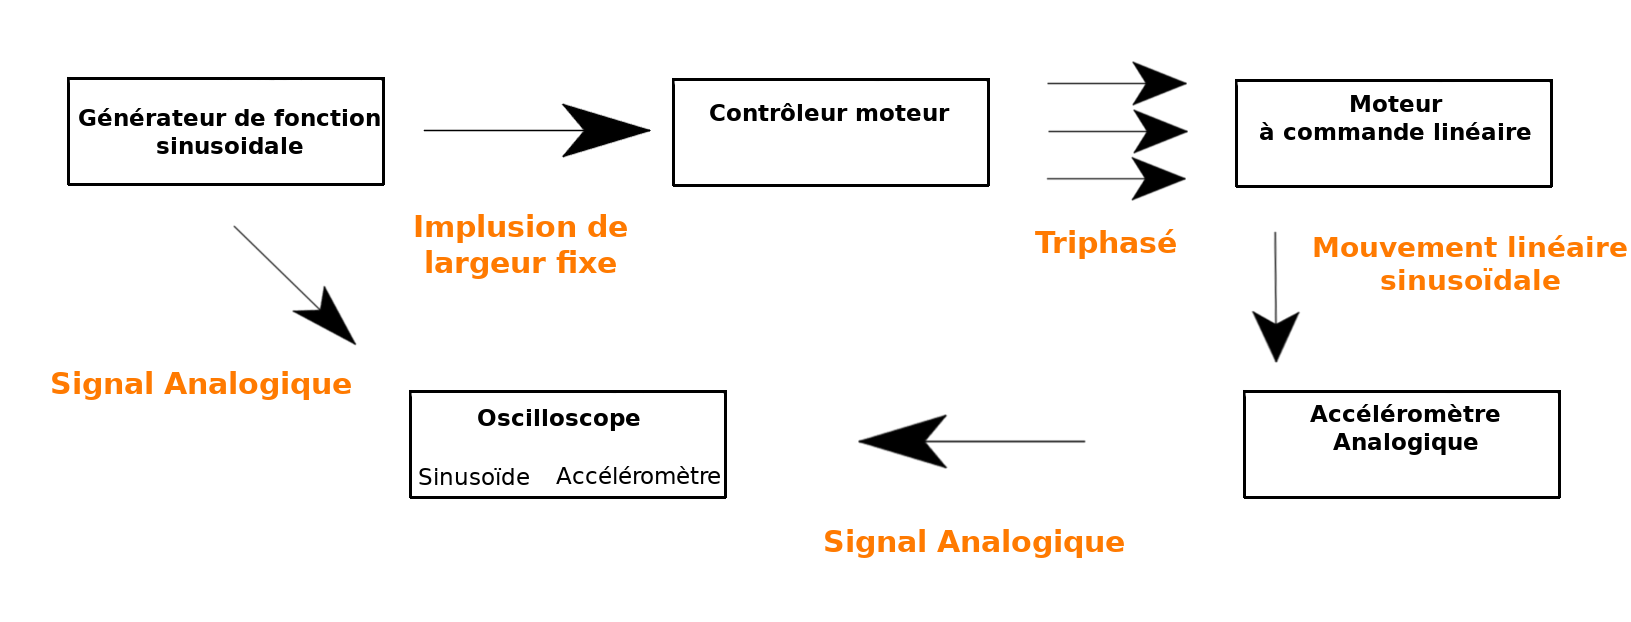
\includegraphics[width=18cm]{manip2.png}
    \caption{Schéma bloc - Seconde manipulation}
	\end{figure}	
		
	
	
	


	
	
	
	
	
	
	
	
	
%--------------------------------------------------------------------------------------
%
%	Elément de fin de document
%		Bibliographie
%		Table des figures
%
%--------------------------------------------------------------------------------------

\part{Bibliographie}

	\begin{itemize}
		\item Descriptif global du projet: BHLS-CNRS-UPMC-LPNHE-IRCAM.pdf
	\end{itemize}


\part{Table des figures}

	\listoffigures



\end{document}